\documentclass[11pt]{article}
\usepackage[a4paper,margin=1in]{geometry}
\usepackage{graphicx}
\usepackage{hyperref}
\usepackage{xcolor}
\usepackage{amsmath}
\usepackage{fancyhdr}
\usepackage{enumitem}
\usepackage{listings}
\usepackage{caption}
\usepackage{titlesec}
\usepackage{float} % Add this to your preamble

\titleformat{\section}{\normalfont\Large\bfseries}{\thesection}{1em}{}
\pagestyle{fancy}
\fancyhf{}
\setlength{\headheight}{13.6pt} % Adjust head height to avoid fancyhdr warning
\rhead{ChiByEye}
\lhead{User Documentation}
\rfoot{\thepage}

\title{\textbf{ChiByEye: An Interactive XSPEC Model Visualizer}}
\author{Paulo Silva \& Paul Draghis}
\date{}

\begin{document}

\maketitle

\section*{Overview}

\textbf{ChiByEye} is an interactive graphical interface built with PyQt5 and Matplotlib that allows users to explore how XSPEC model parameters affect the resulting spectral shape. It provides dynamic visualization, easy model loading, parameter manipulation through sliders or textboxes, and integrated data fitting.

This tool is ideal for astrophysics researchers or students looking to understand model behavior or inspect XSPEC fitting results without manually entering commands in the XSPEC terminal.

\section*{Requirements}

\begin{itemize}
    \item Python 3.x
    \item \textbf{XSPEC} and the \texttt{pyxspec} Python bindings (part of HEASoft)
    \item Python packages:
    \begin{itemize}
        \item \texttt{numpy}
        \item \texttt{matplotlib}
        \item \texttt{PyQt5}
    \end{itemize}
\end{itemize}

\noindent
Additionally, the code attempts to load the \texttt{relxill} model on startup. If your system does not have \texttt{relxill} installed, comment out \texttt{AllModels.lmod('relxill')} (line 38).

\section*{Launching the Interface}

After installing the dependencies and verifying XSPEC is properly configured, run the software with:

\begin{lstlisting}[language=bash]
python xspec_plot_interface.py
\end{lstlisting}

\section*{Main Interface}

\begin{figure}[H]
    \centering
    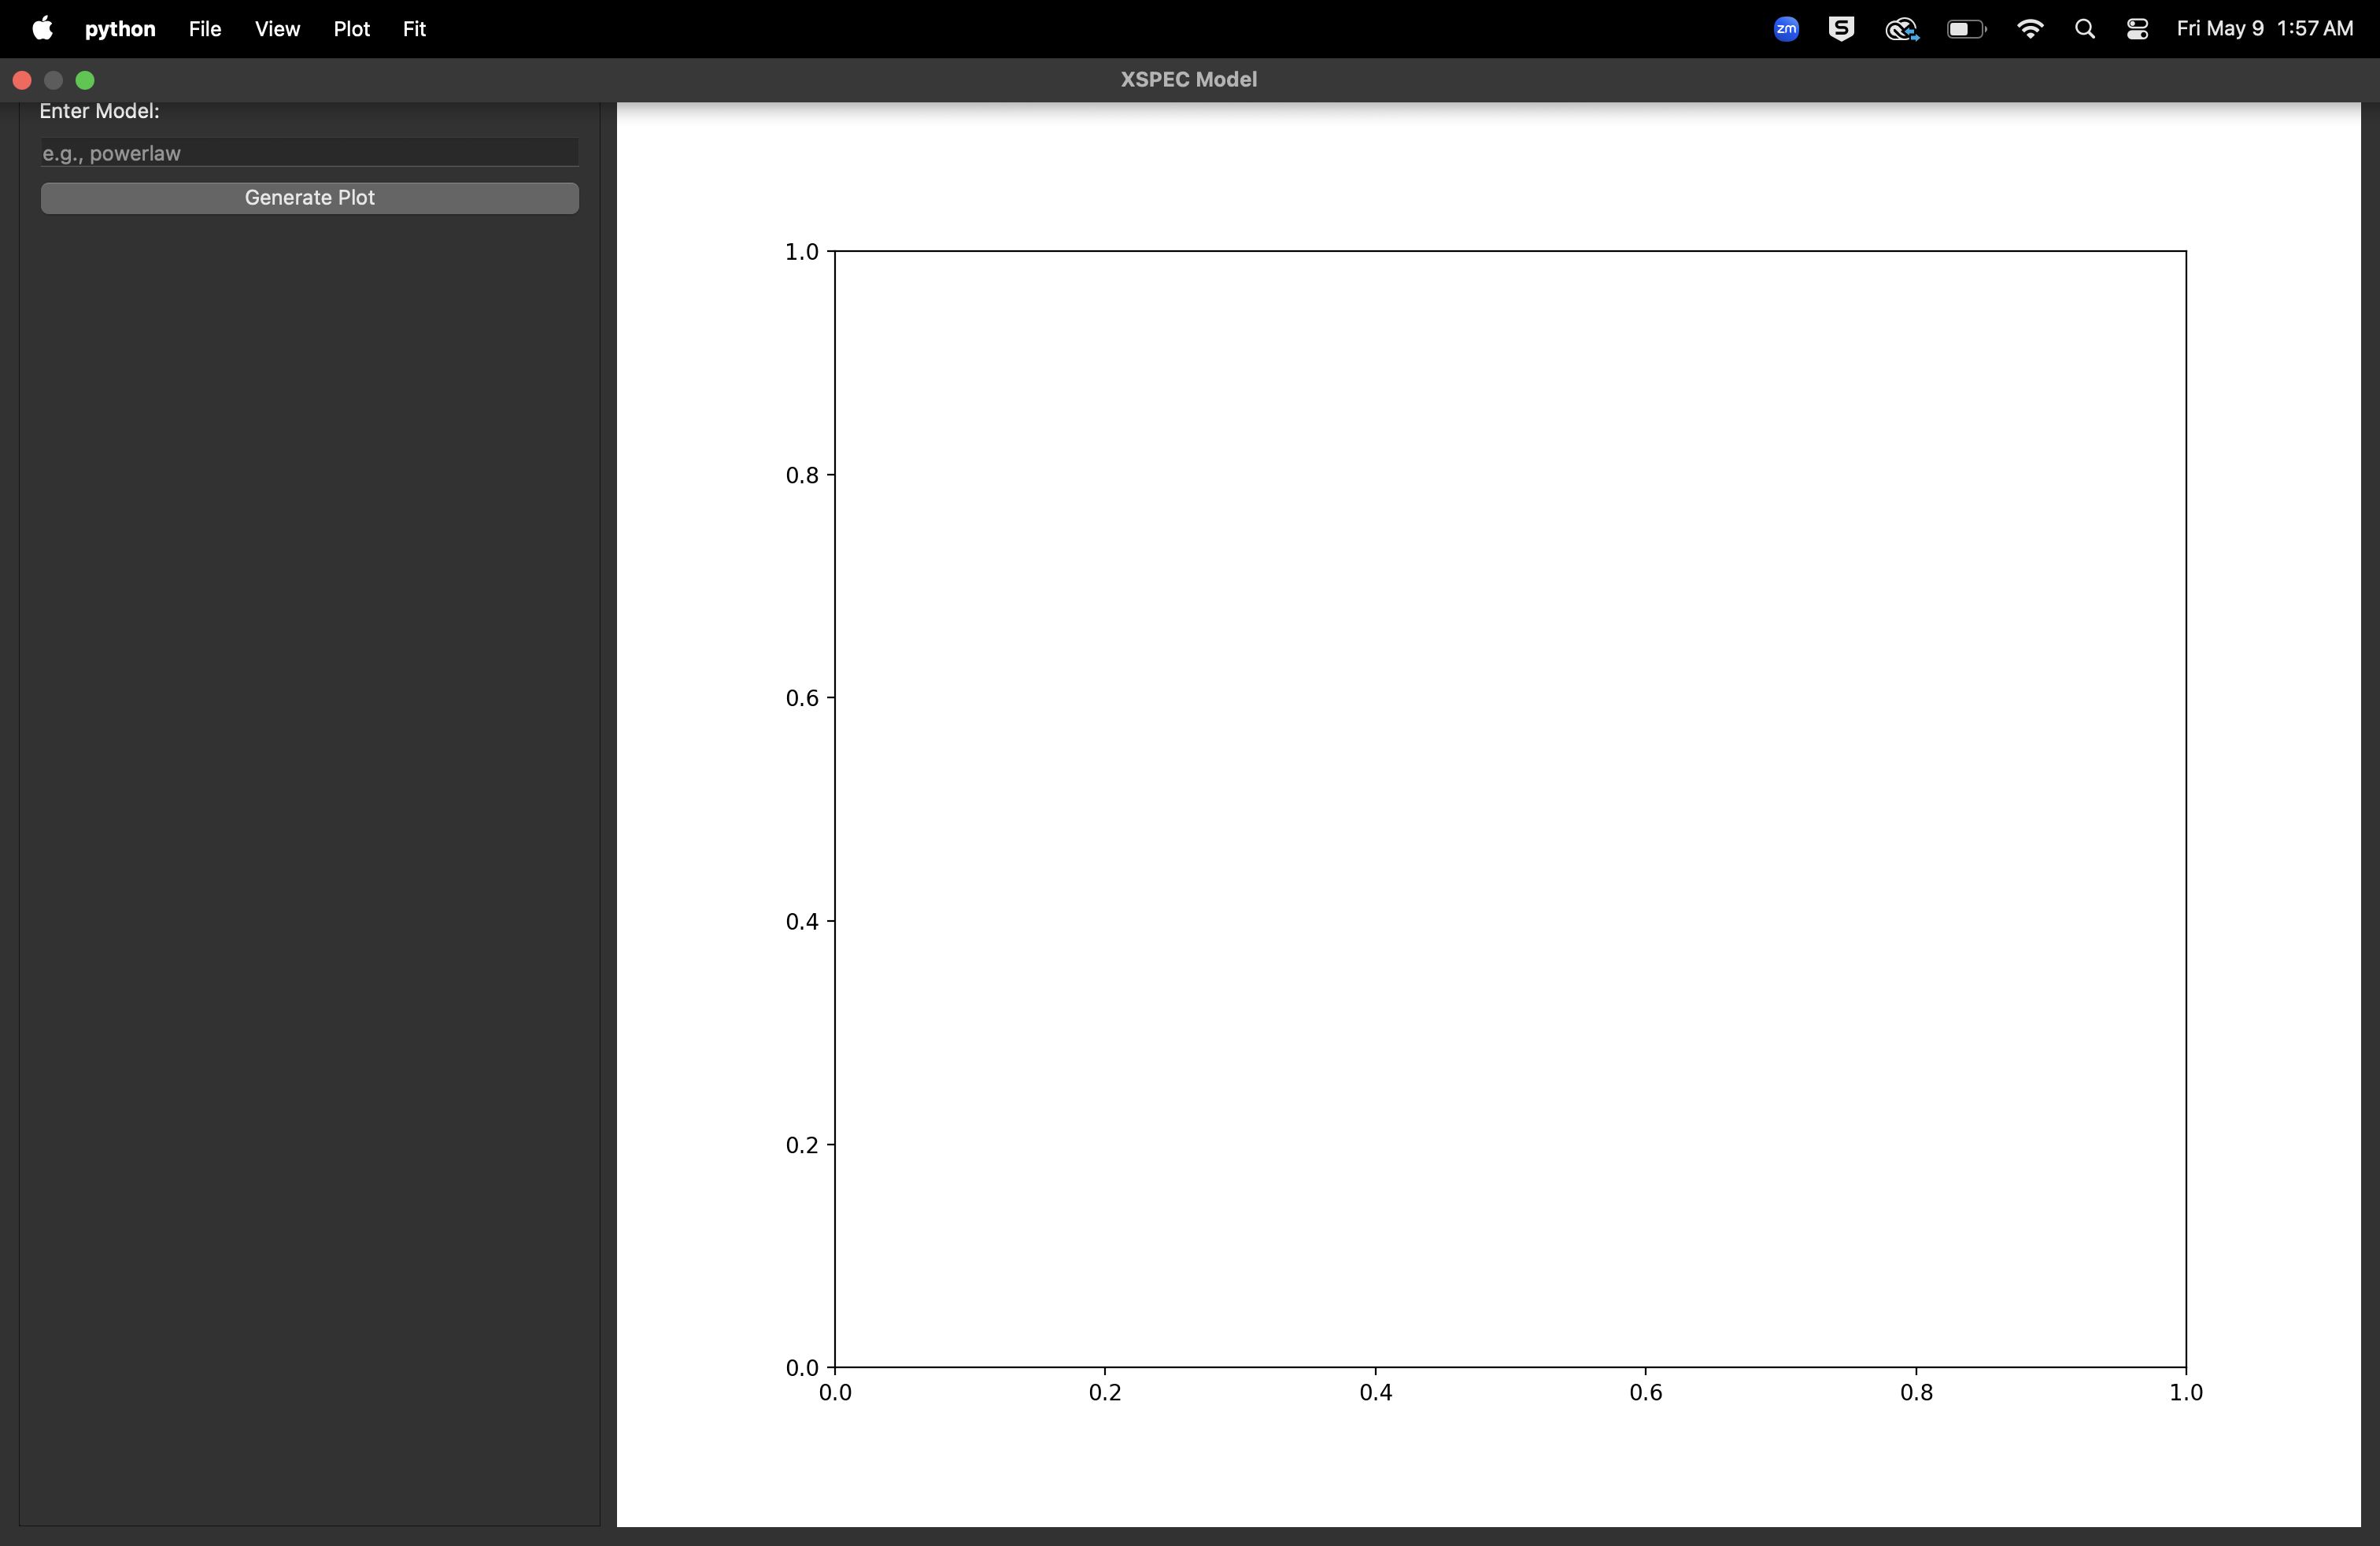
\includegraphics[width=0.7\linewidth]{documentation_images/initial_screen.png}
    \caption{The initial ChiByEye interface upon launch.}
\end{figure}

\begin{itemize}
    \item \textbf{Manual model entry:} Type the model expression and press \texttt{Enter}.
    \item \textbf{File $\rightarrow$ Load Model as XCM:} Load a model from an existing \texttt{.xcm} file.
    \item \textbf{File $\rightarrow$ Load Data as XCM:} Load both spectra and model from an XSPEC session file.
\end{itemize}


\begin{figure}[H]
    \centering
    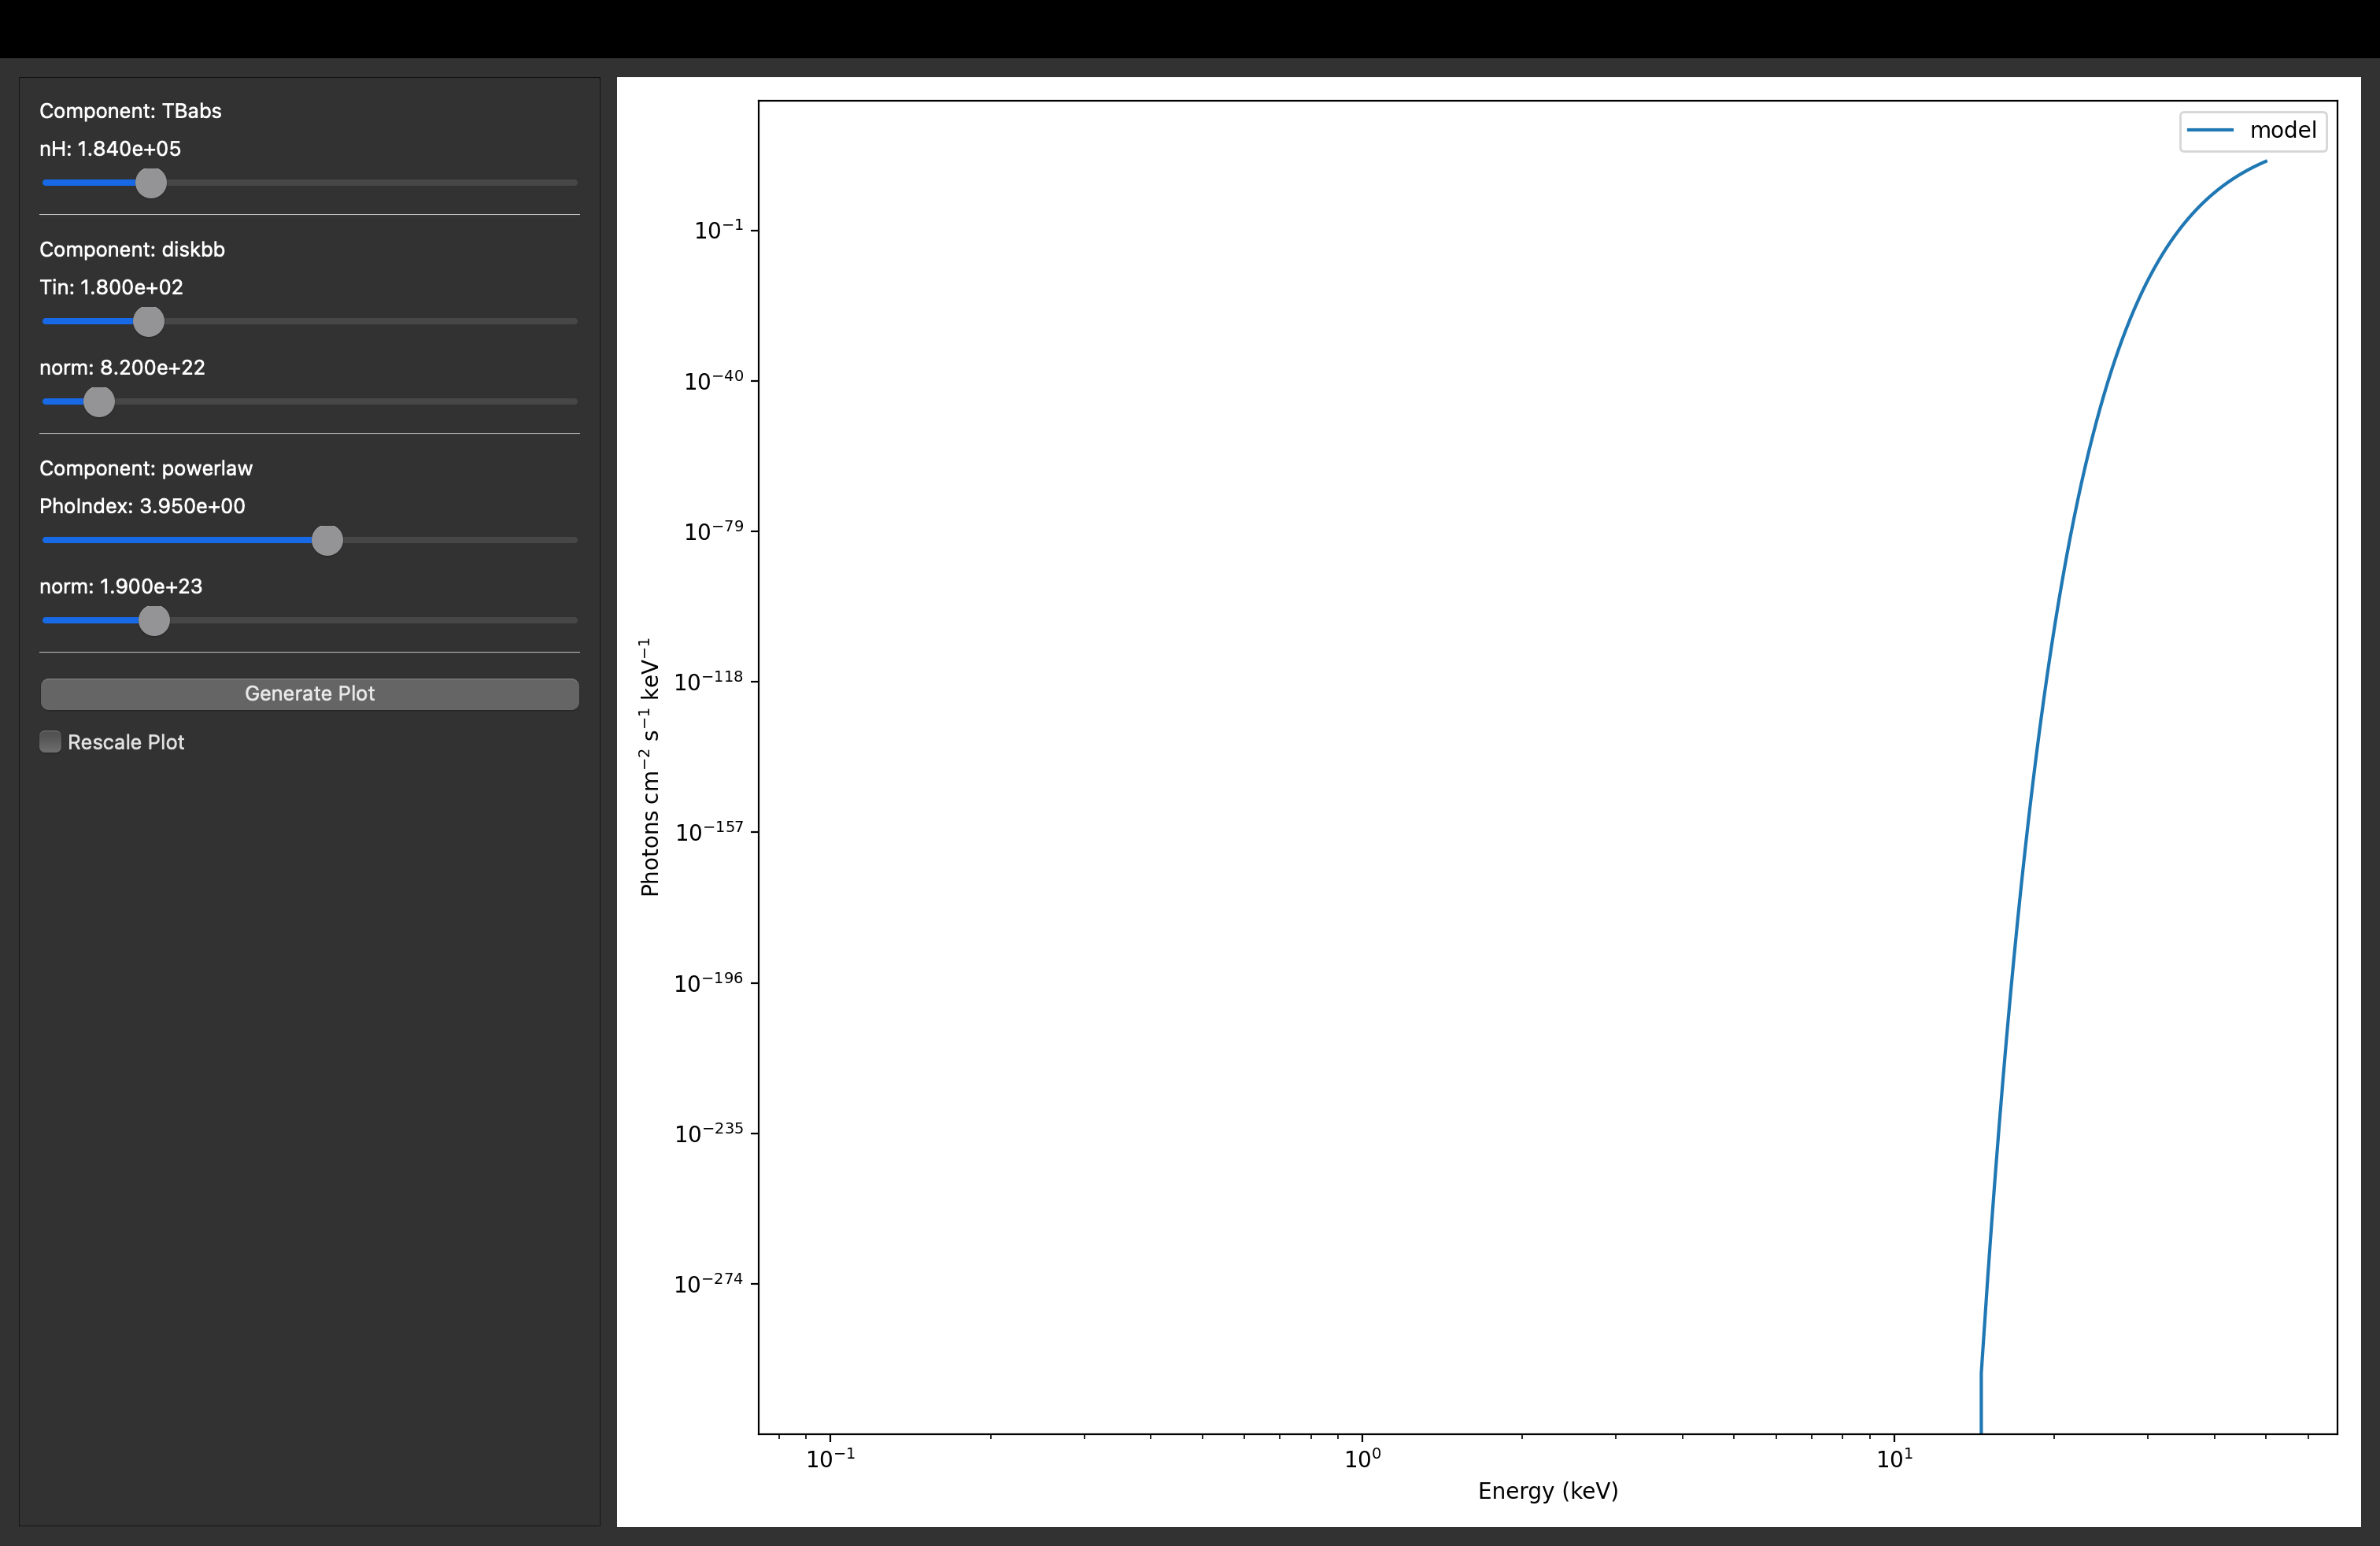
\includegraphics[width=0.7\linewidth]{documentation_images/plot_after_changing_sliders.png}
    \caption{Model plot after adjusting parameters using sliders.}
\end{figure}

\begin{figure}[H]
    \centering
    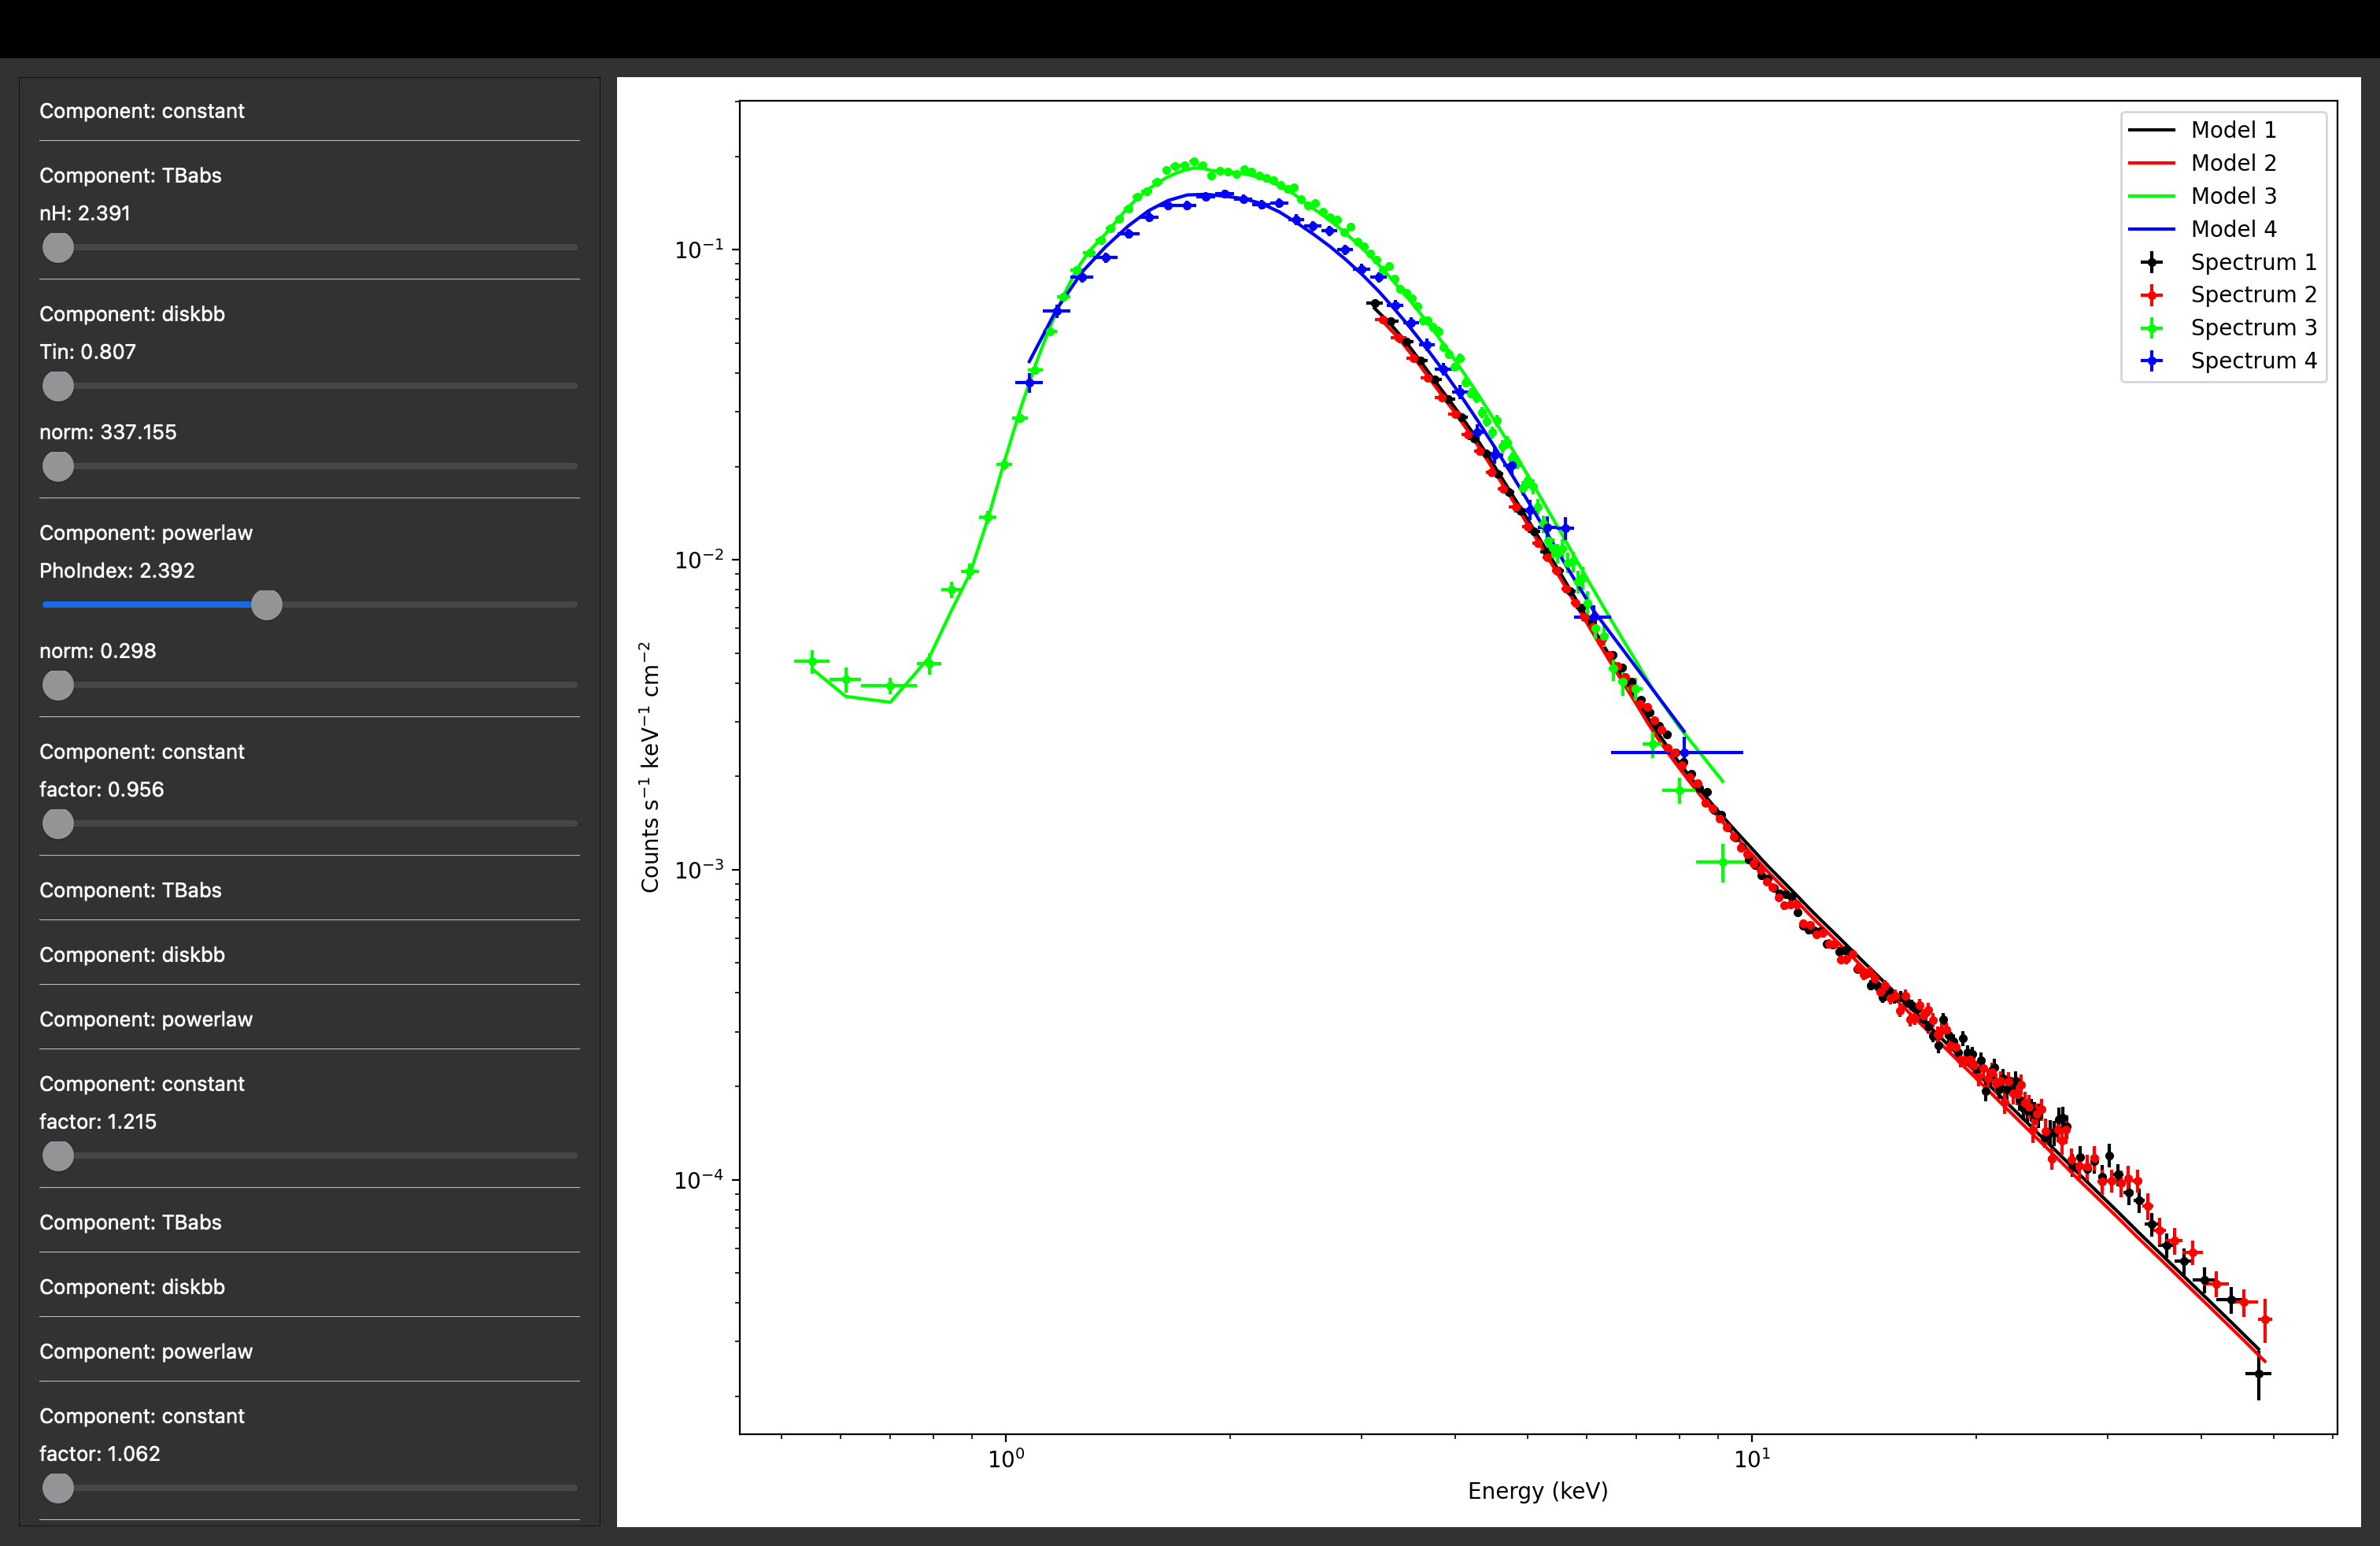
\includegraphics[width=0.7\linewidth]{documentation_images/load_data_as_xcm.png}
    \caption{Loading data and model from an XSPEC .xcm session file.}
\end{figure}

\noindent
An example XCM file (\texttt{test\_file.xcm}) is provided to demonstrate functionality.

\section*{View Menu Options}

\begin{itemize}
    \item \textbf{Use Textboxes for Parameters:} Toggles between sliders and textboxes for editing model parameters.
    \item \textbf{Set Axes Limits:} Manually define x and y-axis limits for the plot.
    \item \textbf{Freeze Axes:} Lock current axis limits for consistent comparison between plots.
    \item \textbf{Show Frozen Parameters:} Display parameters that are frozen in XSPEC.
\end{itemize}

\begin{figure}[H]
    \centering
    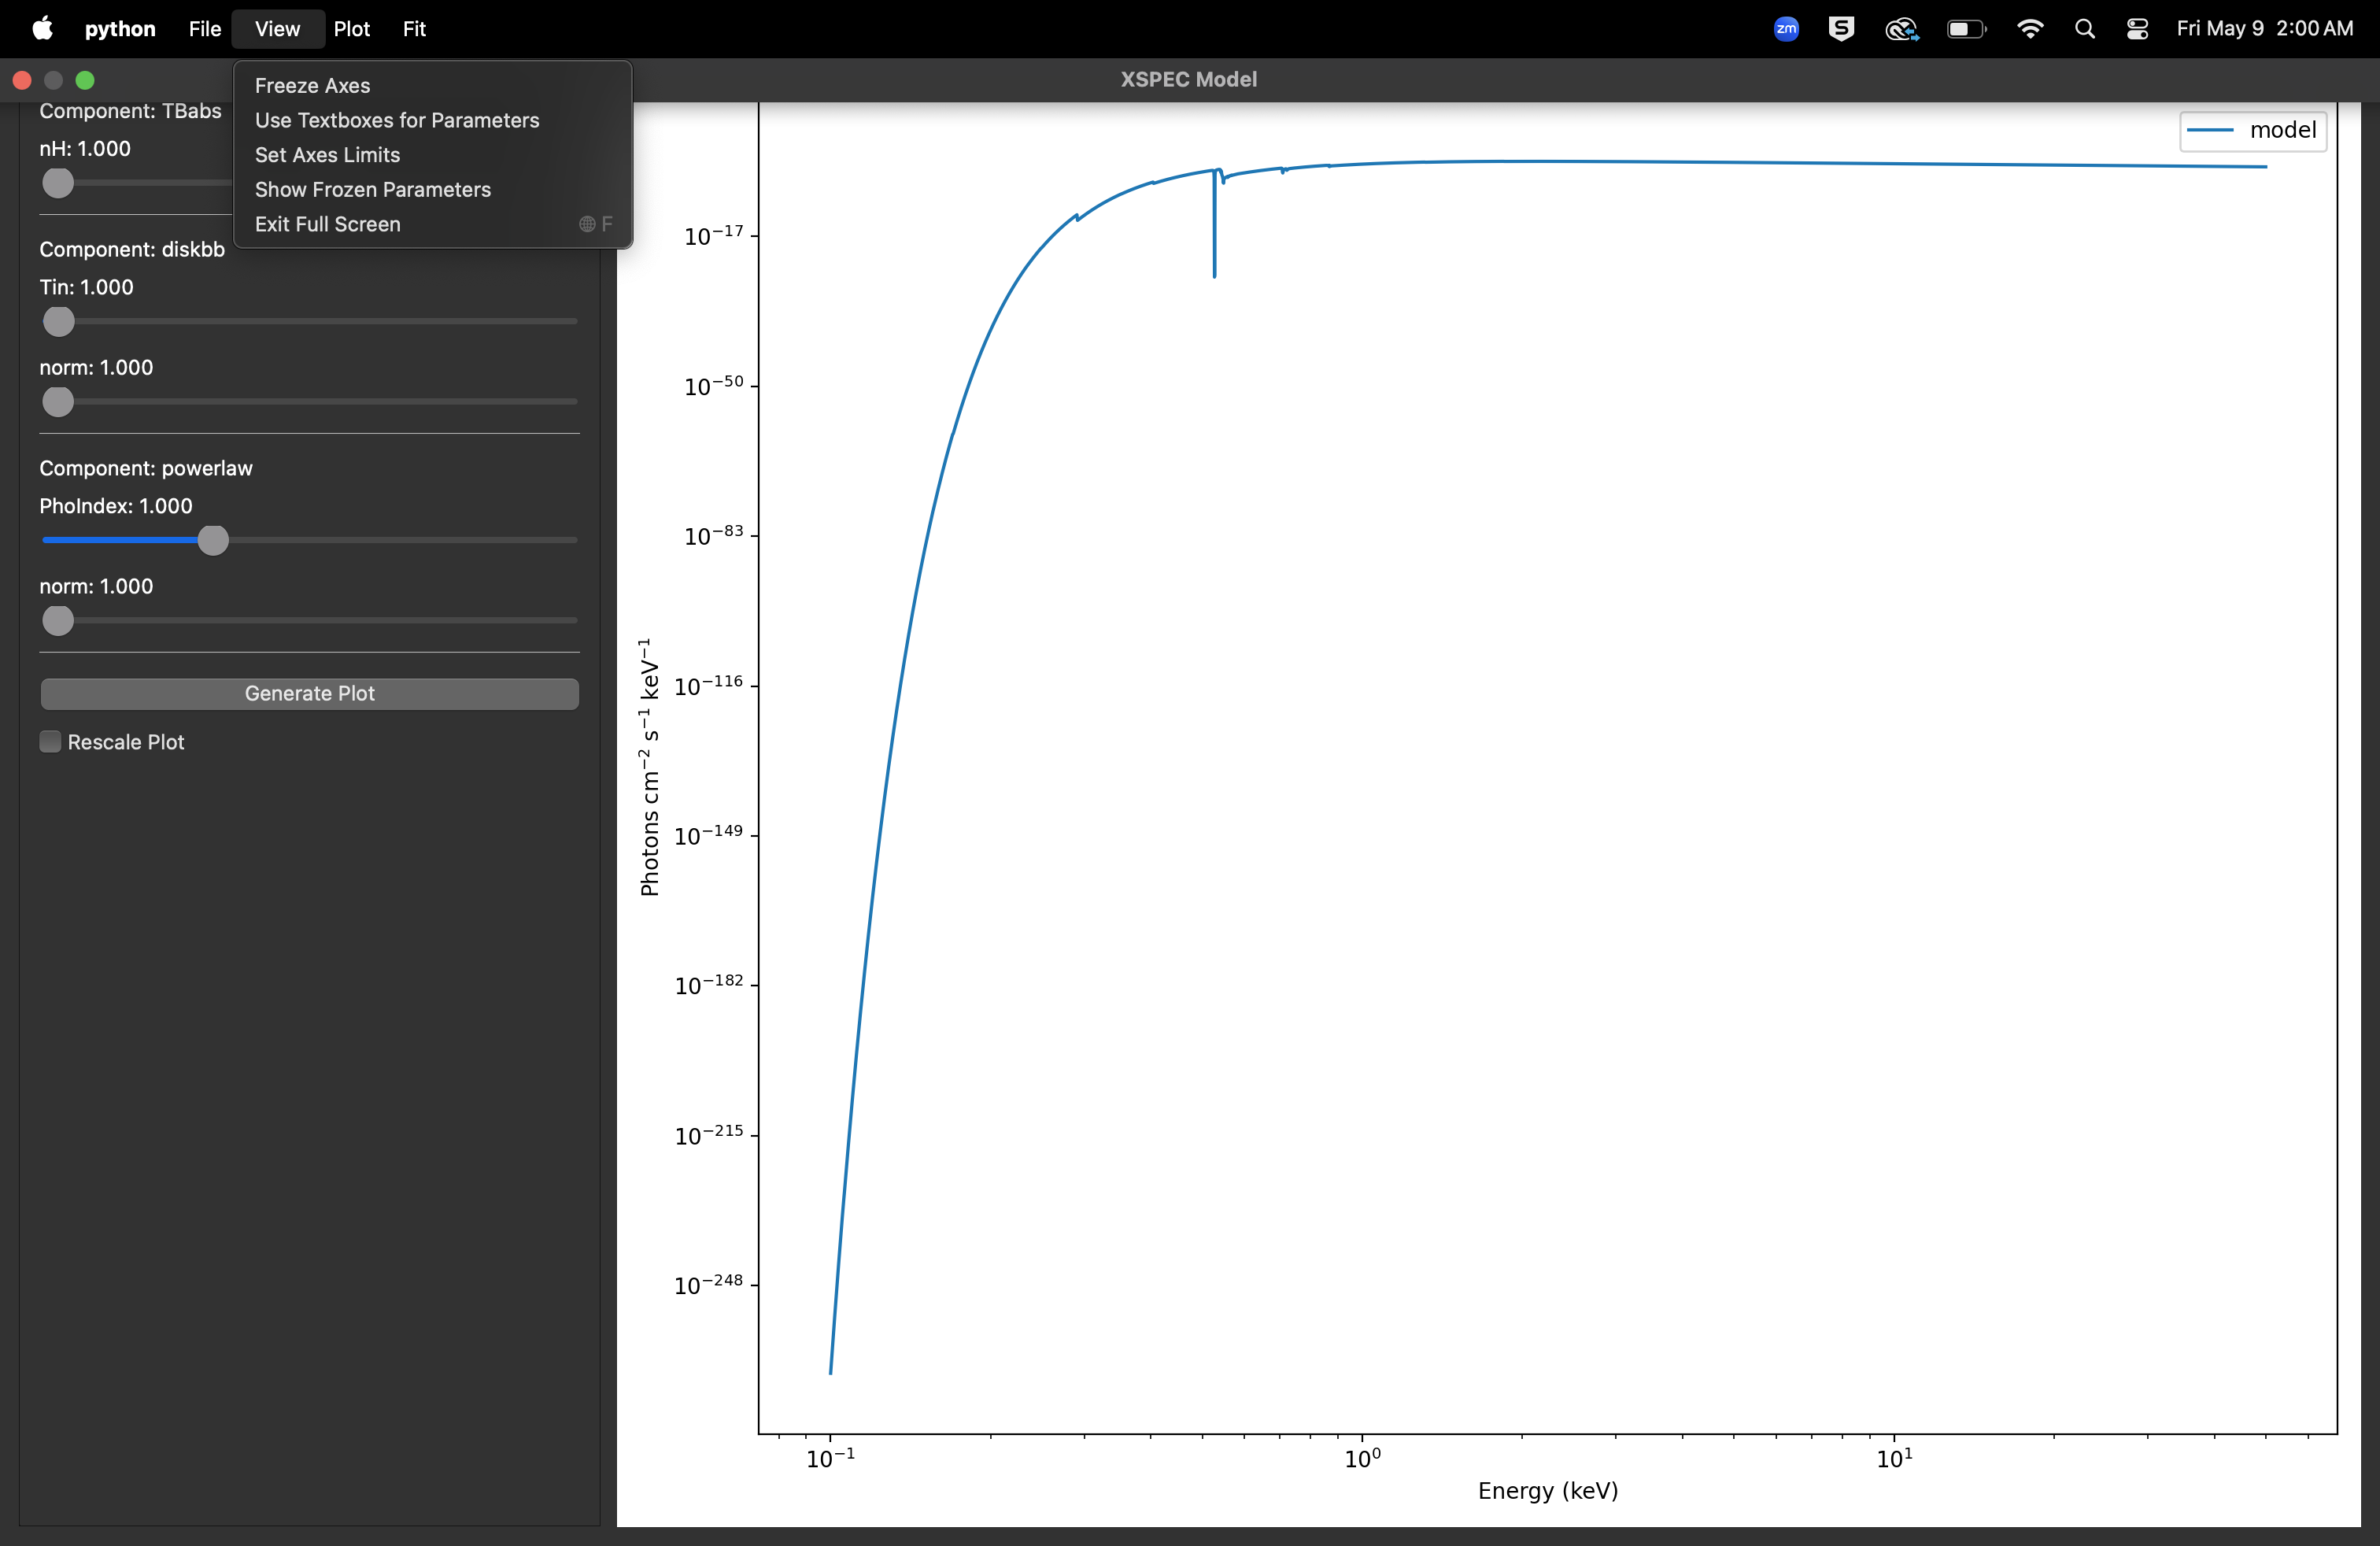
\includegraphics[width=0.7\linewidth]{documentation_images/view_menu.png}
    \caption{The View menu allows toggling interface features and parameter display.}
\end{figure}

\begin{figure}[H]
    \centering
    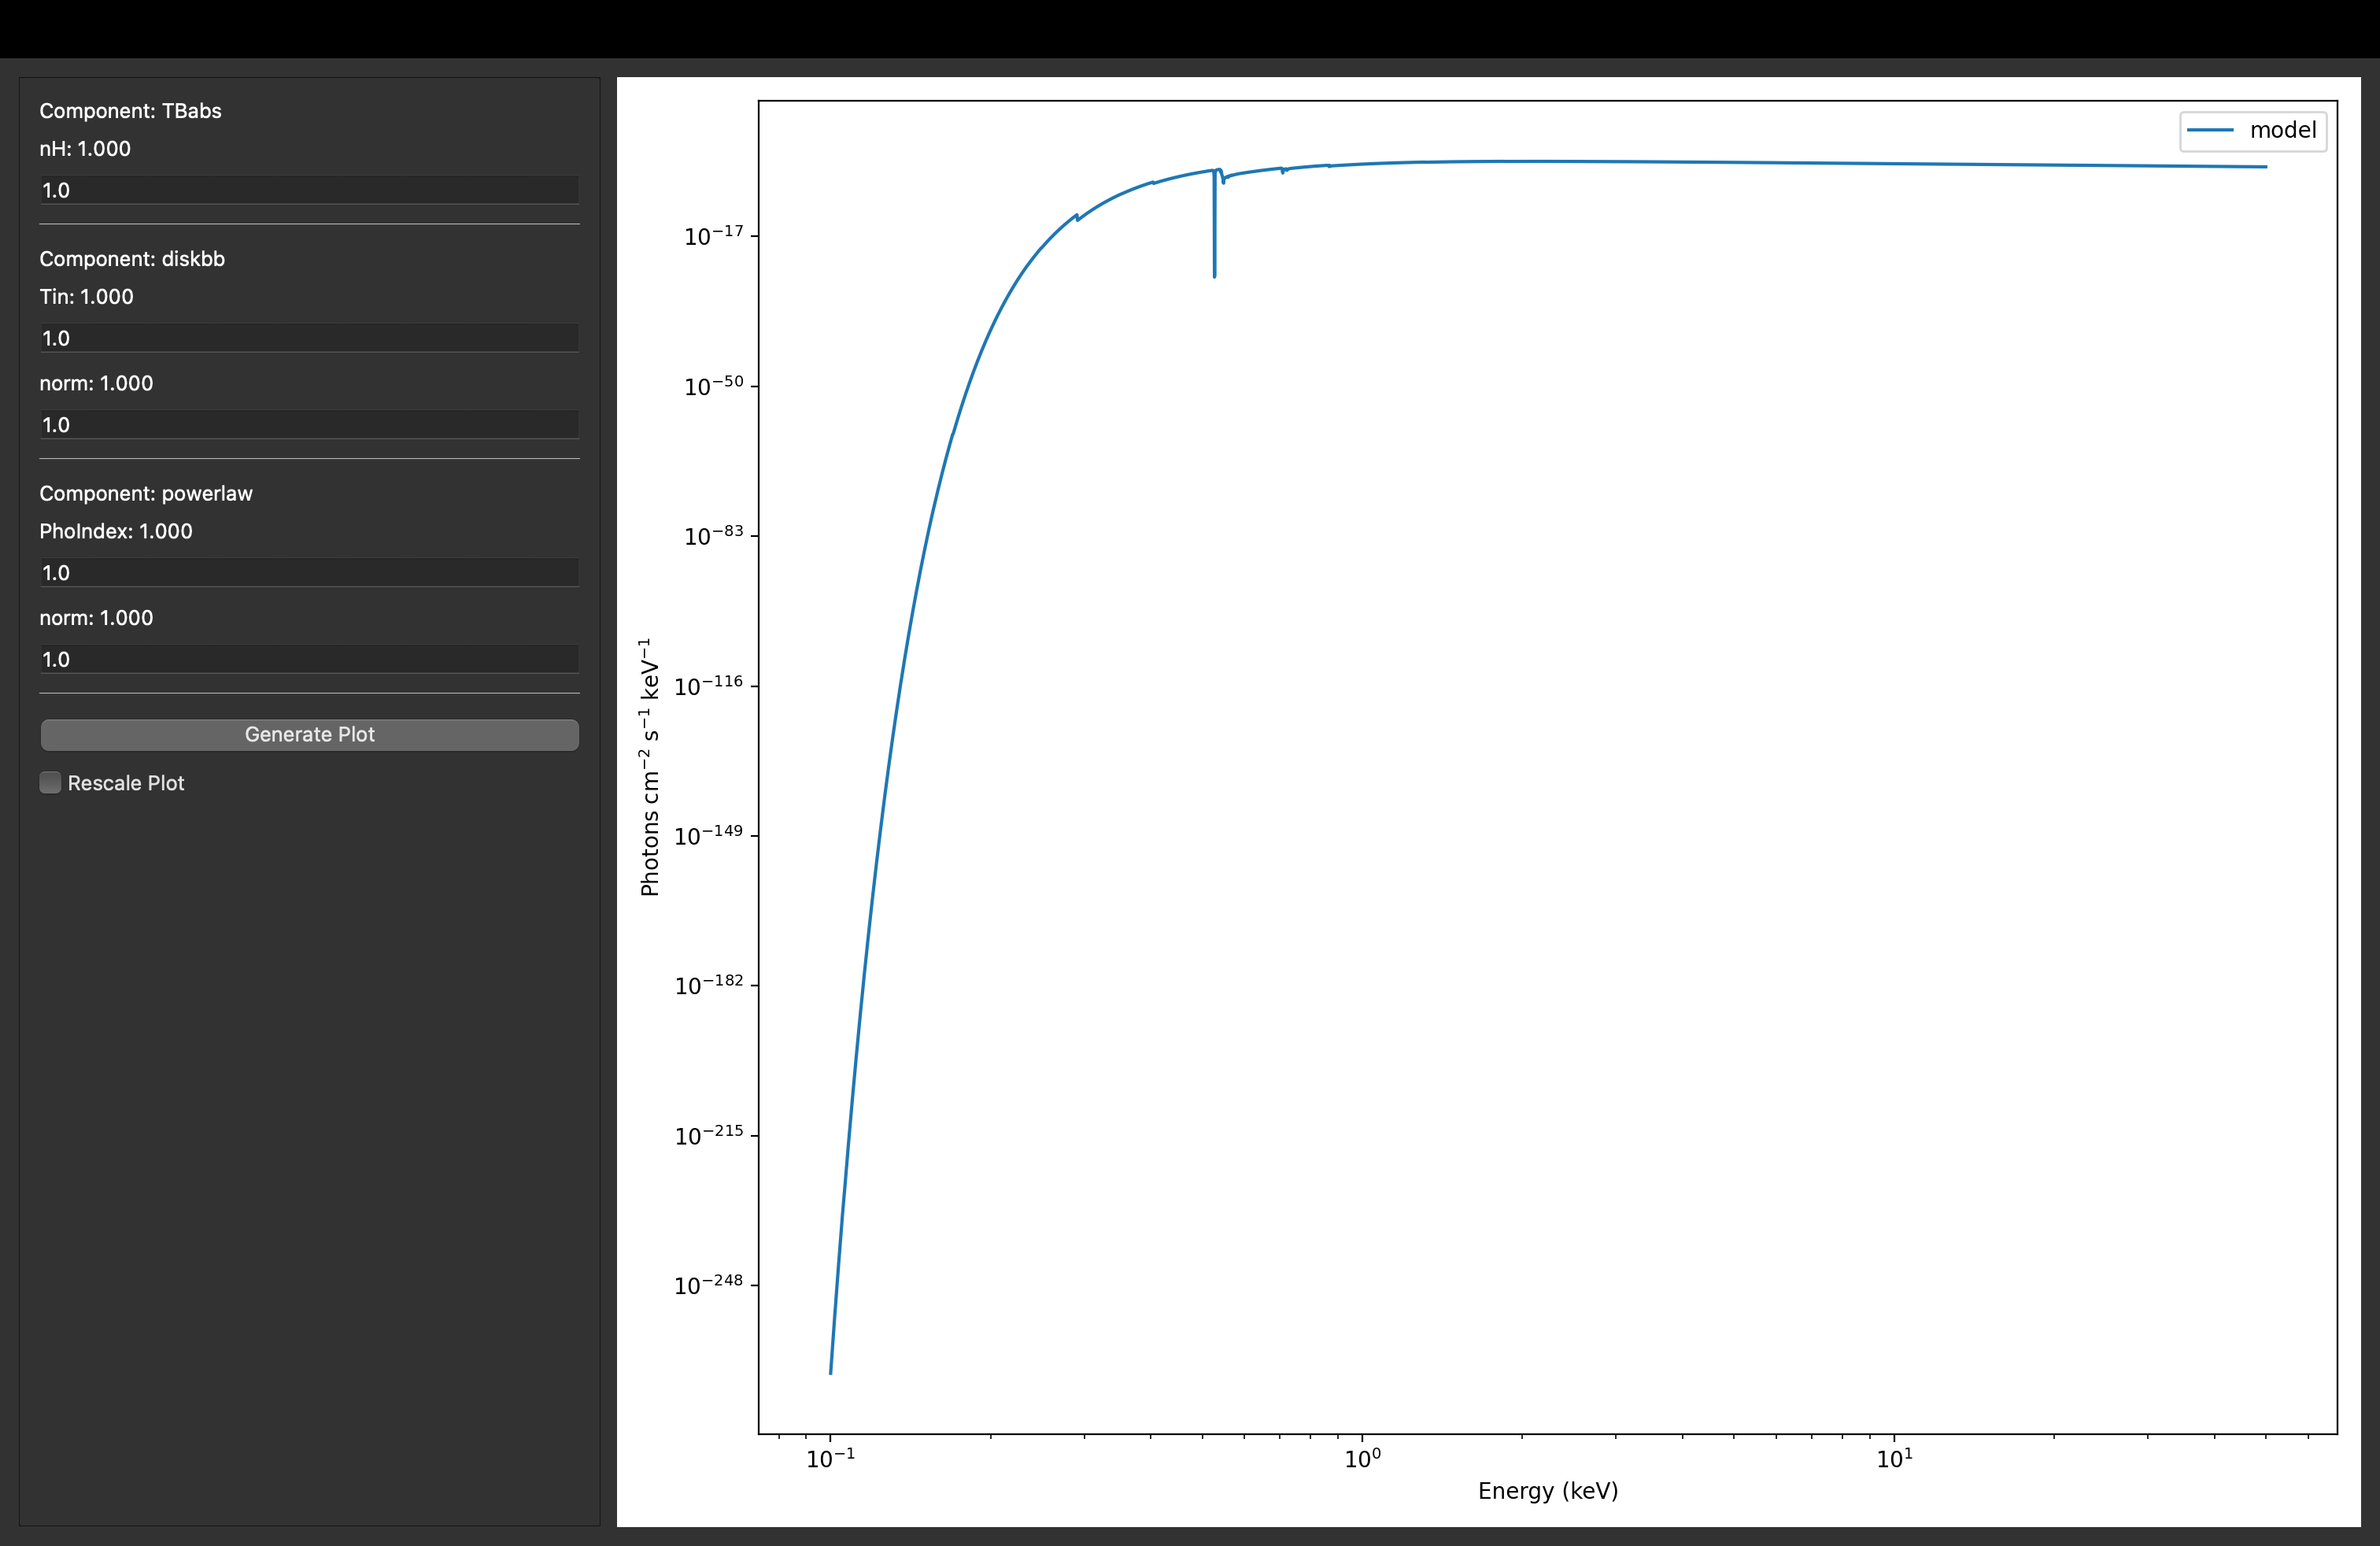
\includegraphics[width=0.7\linewidth]{documentation_images/textboxes.png}
    \caption{Switching between sliders and textboxes for parameter input.}
\end{figure}

\begin{figure}[H]
    \centering
    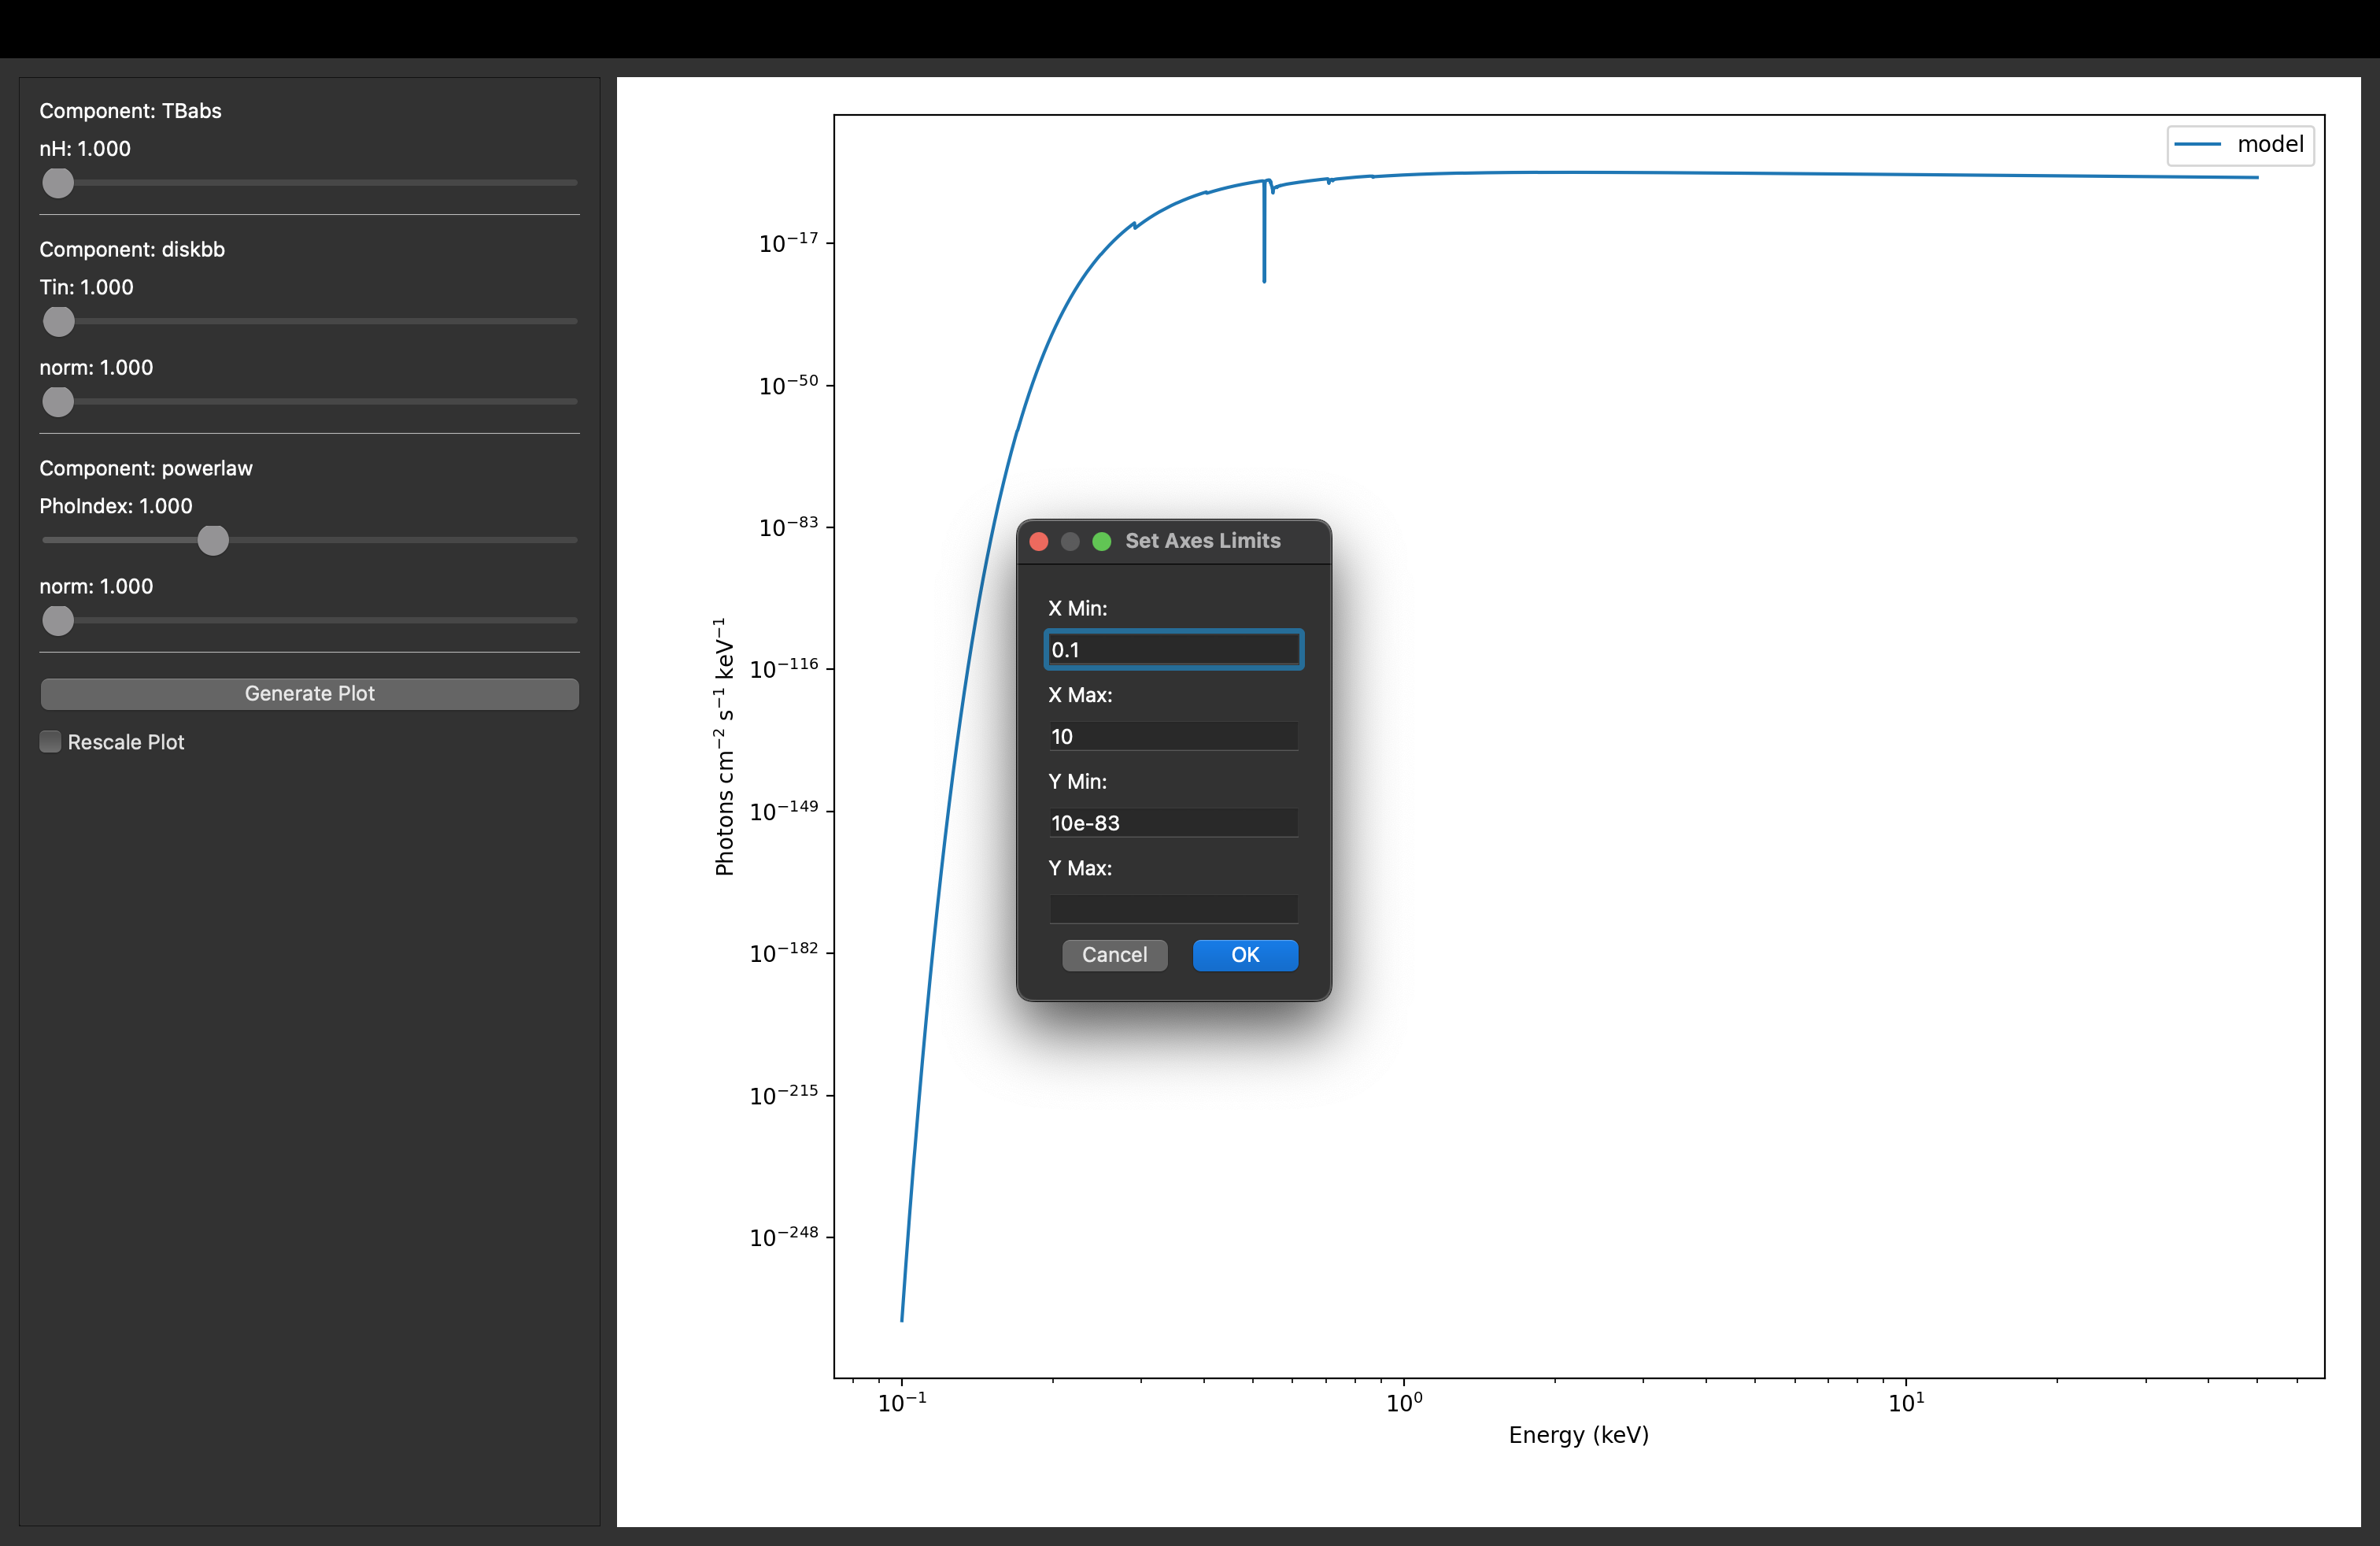
\includegraphics[width=0.7\linewidth]{documentation_images/set_axes_limits.png}
    \caption{Dialog for setting plot axes limits.}
\end{figure}

\section*{Buttons and Controls}

\begin{itemize}
    \item \textbf{Generate Plot:} Refresh the model plot using the current parameters.
    \item \textbf{Rescale Plot (Checkbox):} Rescales the y-axis to focus on relevant data. Useful when plotted values become too small in log space (e.g., $10^{-\infty}$).
\end{itemize}

\section*{Plot Menu Features}

\begin{itemize}
    \item \textbf{Plot Different Components:} Visualize each additive component of a model individually (e.g., diskbb + powerlaw).
    \item \textbf{Plot Model:} Select XSPEC plot styles: \texttt{model}, \texttt{emodel}, \texttt{eemodel}.
    \item \textbf{Plot Data:} Choose from data-only, data+ratio, or unfolded spectrum + delchi representations.
    \item \textbf{Plot Same Curve N Times:} Sweep a parameter across multiple values and show the resulting curves using a color map.
\end{itemize}

\begin{figure}[H]
    \centering
    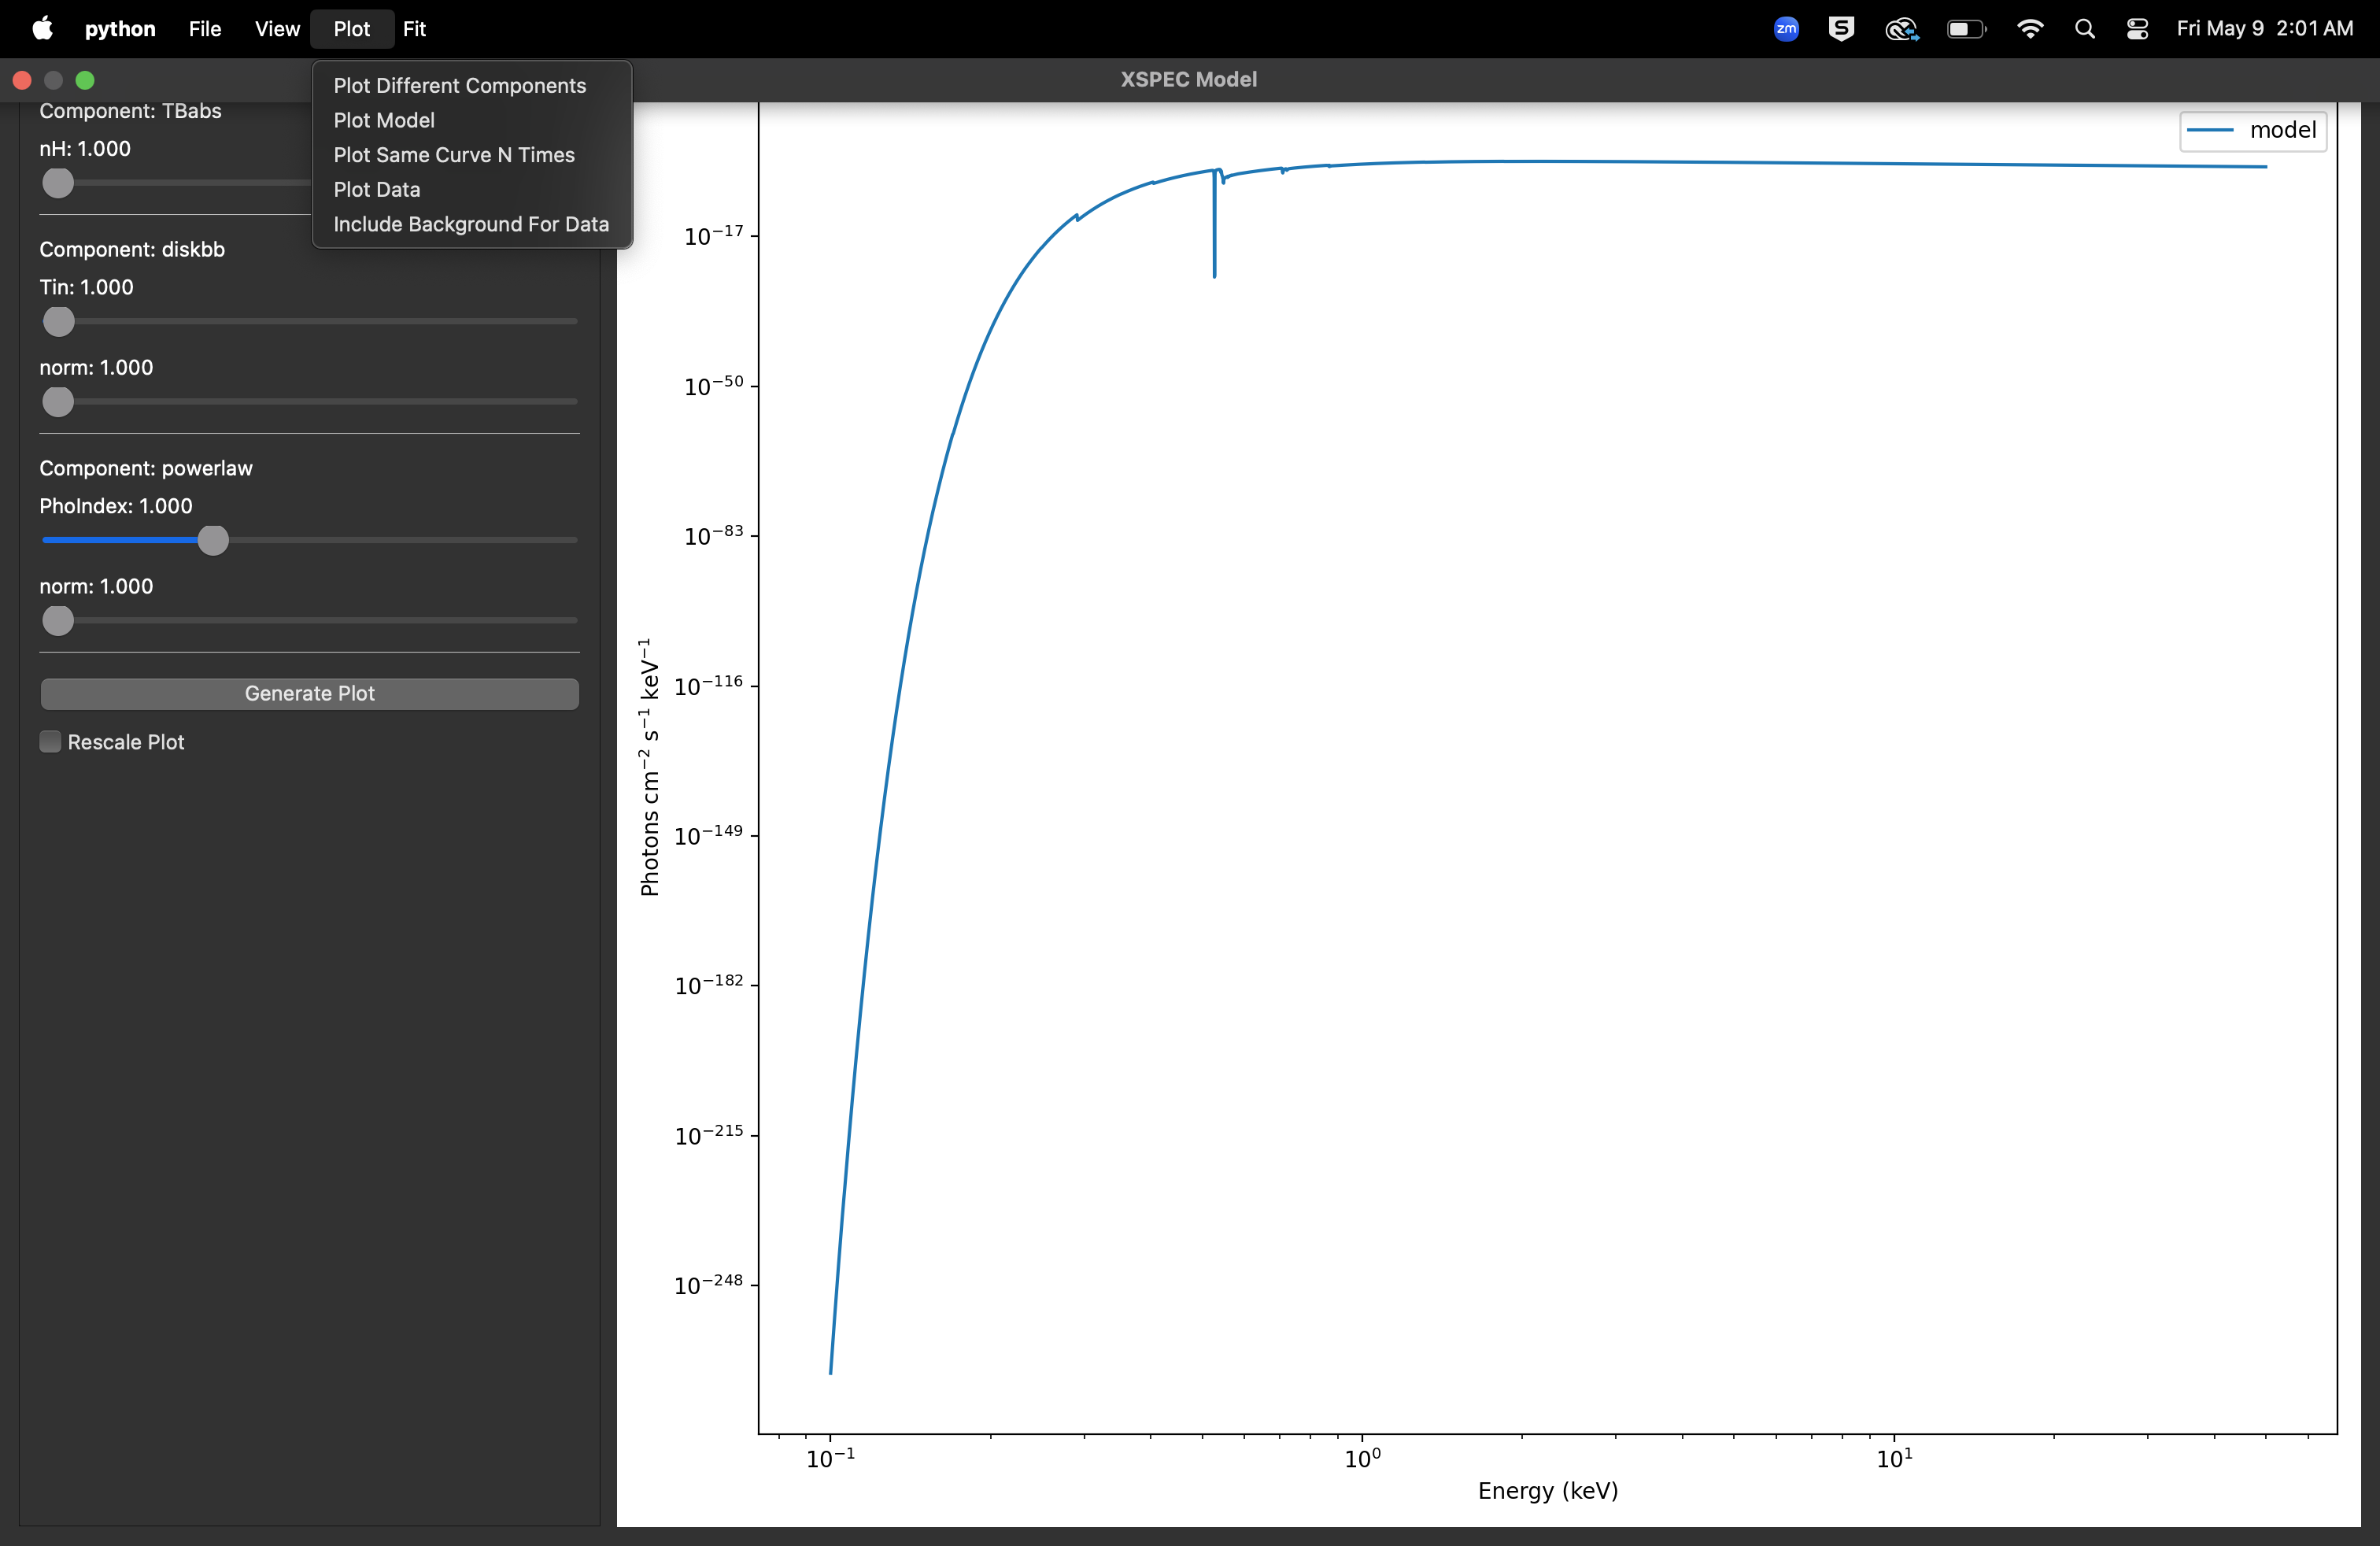
\includegraphics[width=0.7\linewidth]{documentation_images/plot_menu.png}
    \caption{The Plot menu enables selection of plot types and fitting options.}
\end{figure}

\begin{figure}[H]
    \centering
    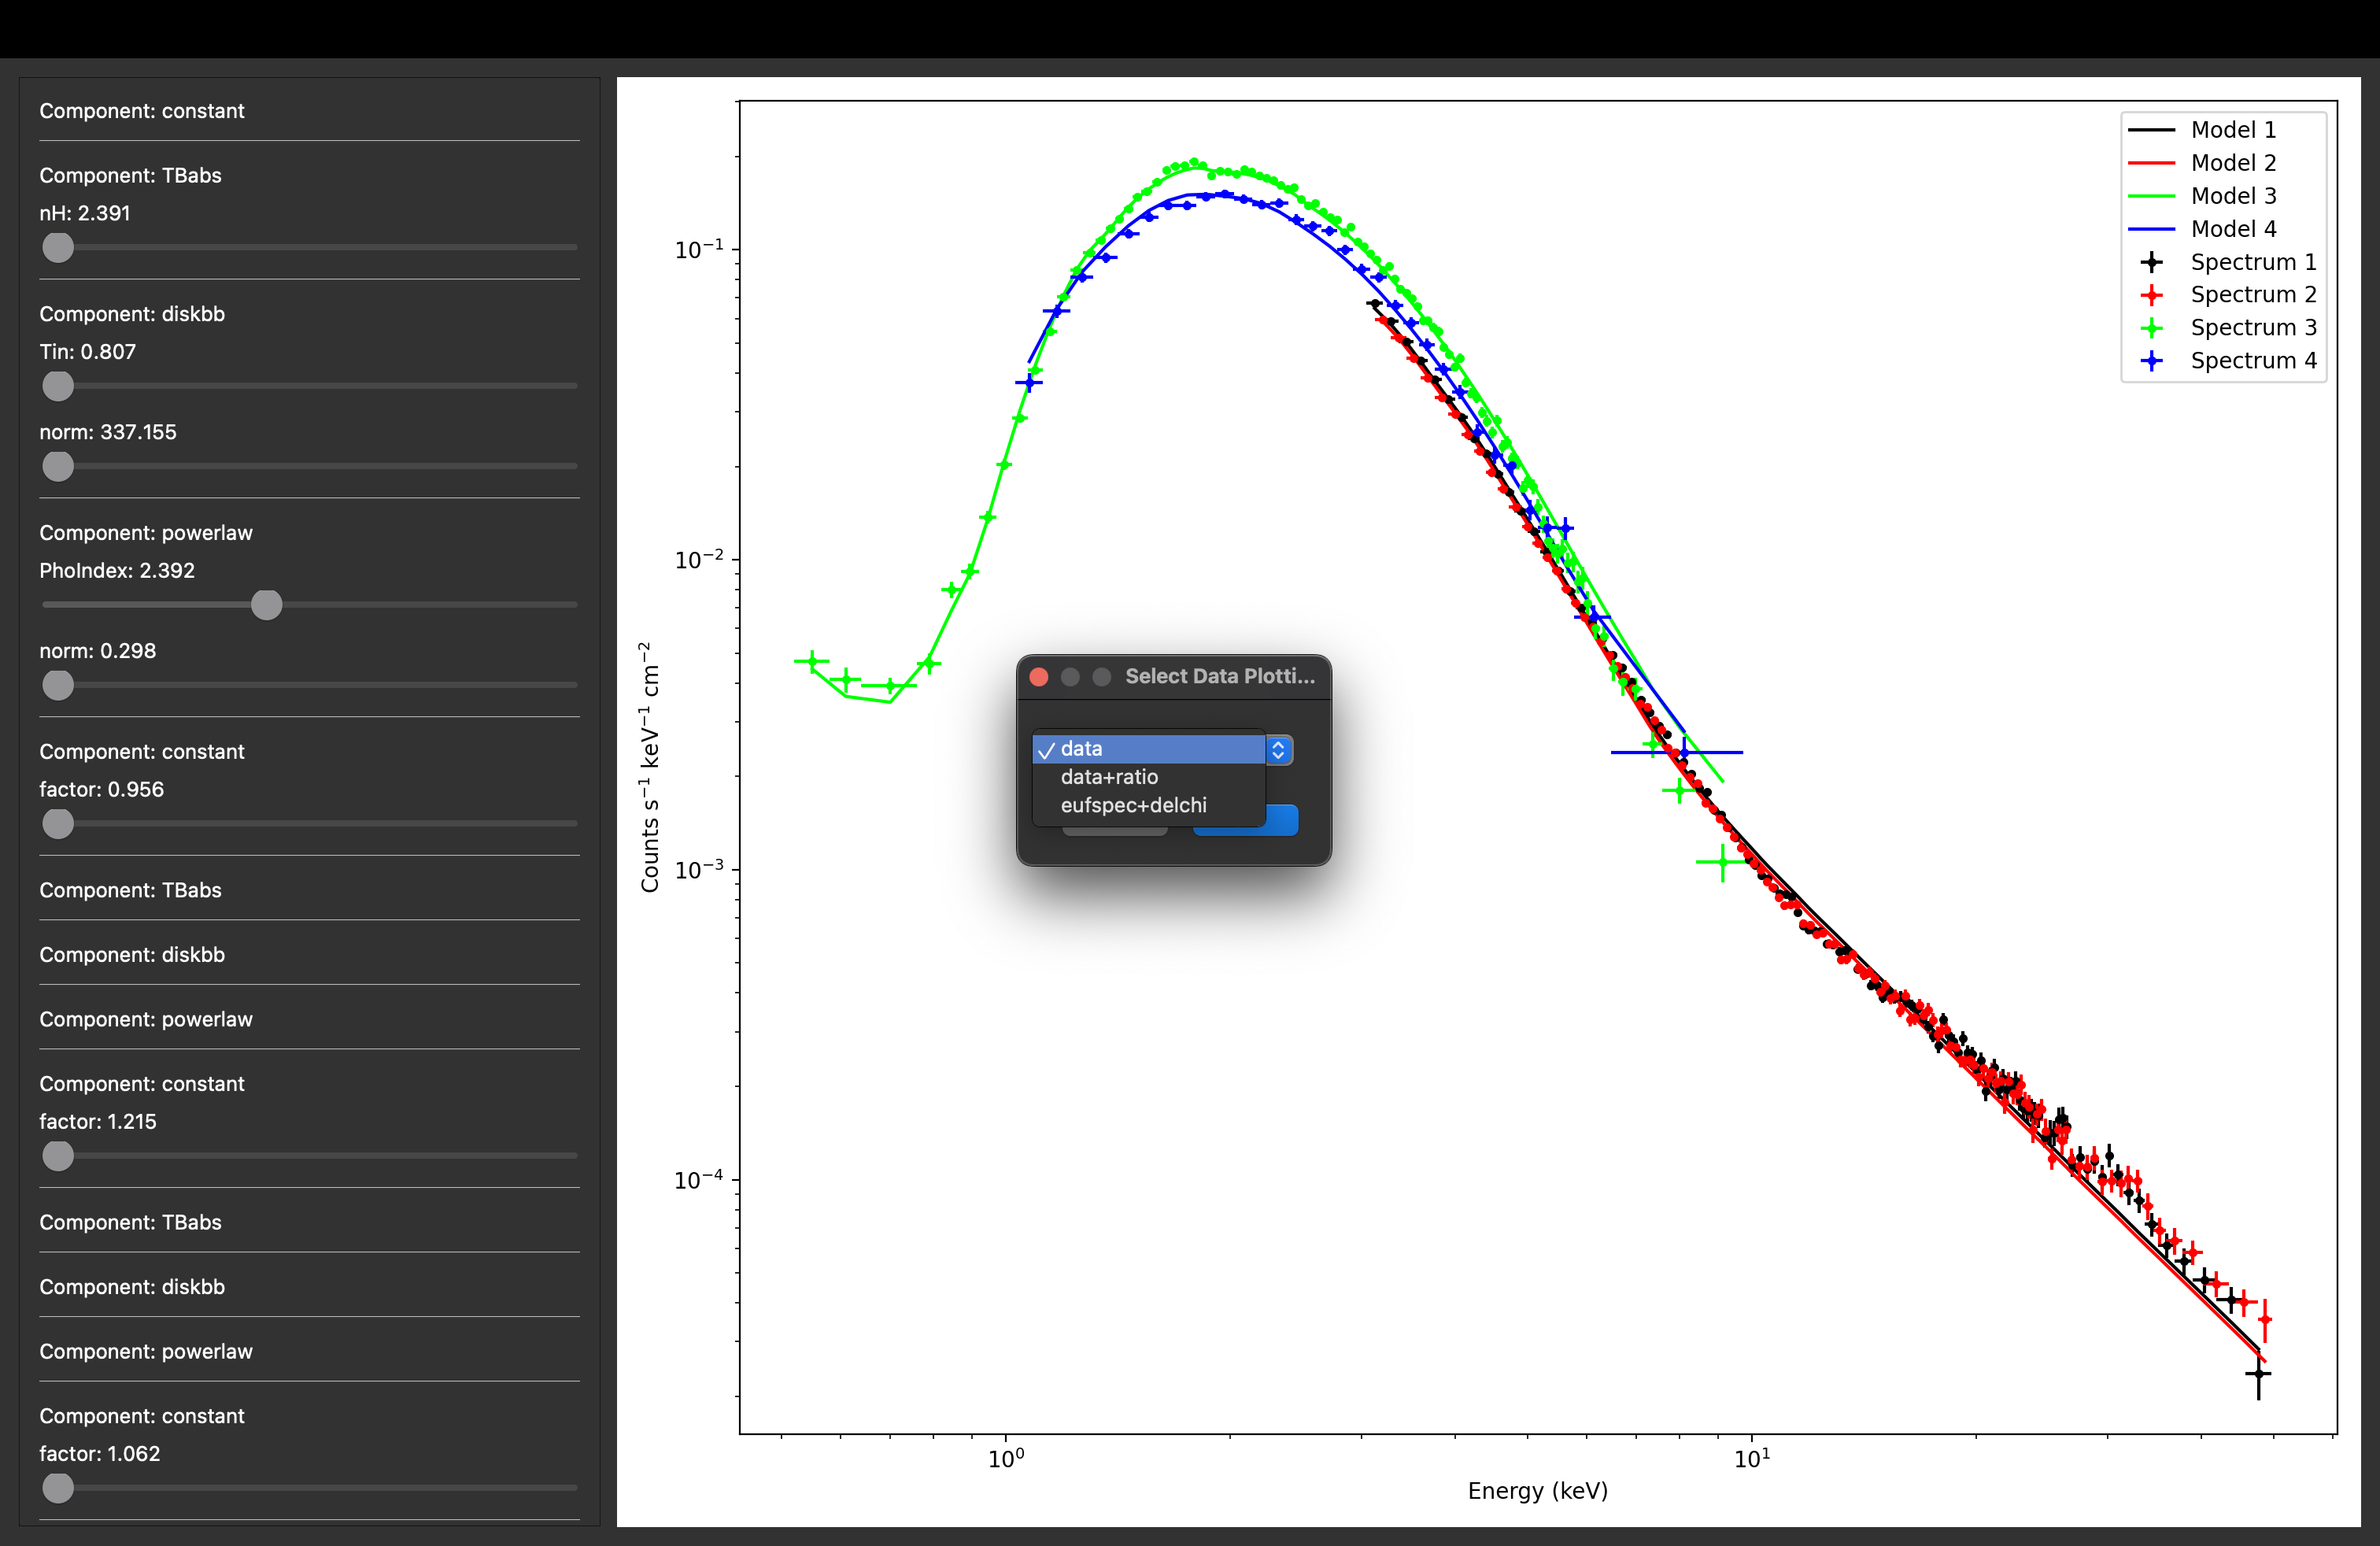
\includegraphics[width=0.7\linewidth]{documentation_images/plot_data-options.png}
    \caption{Different data plot options: data-only, data+ratio, unfolded spectrum + delchi.}
\end{figure}

\begin{figure}[H]
    \centering
    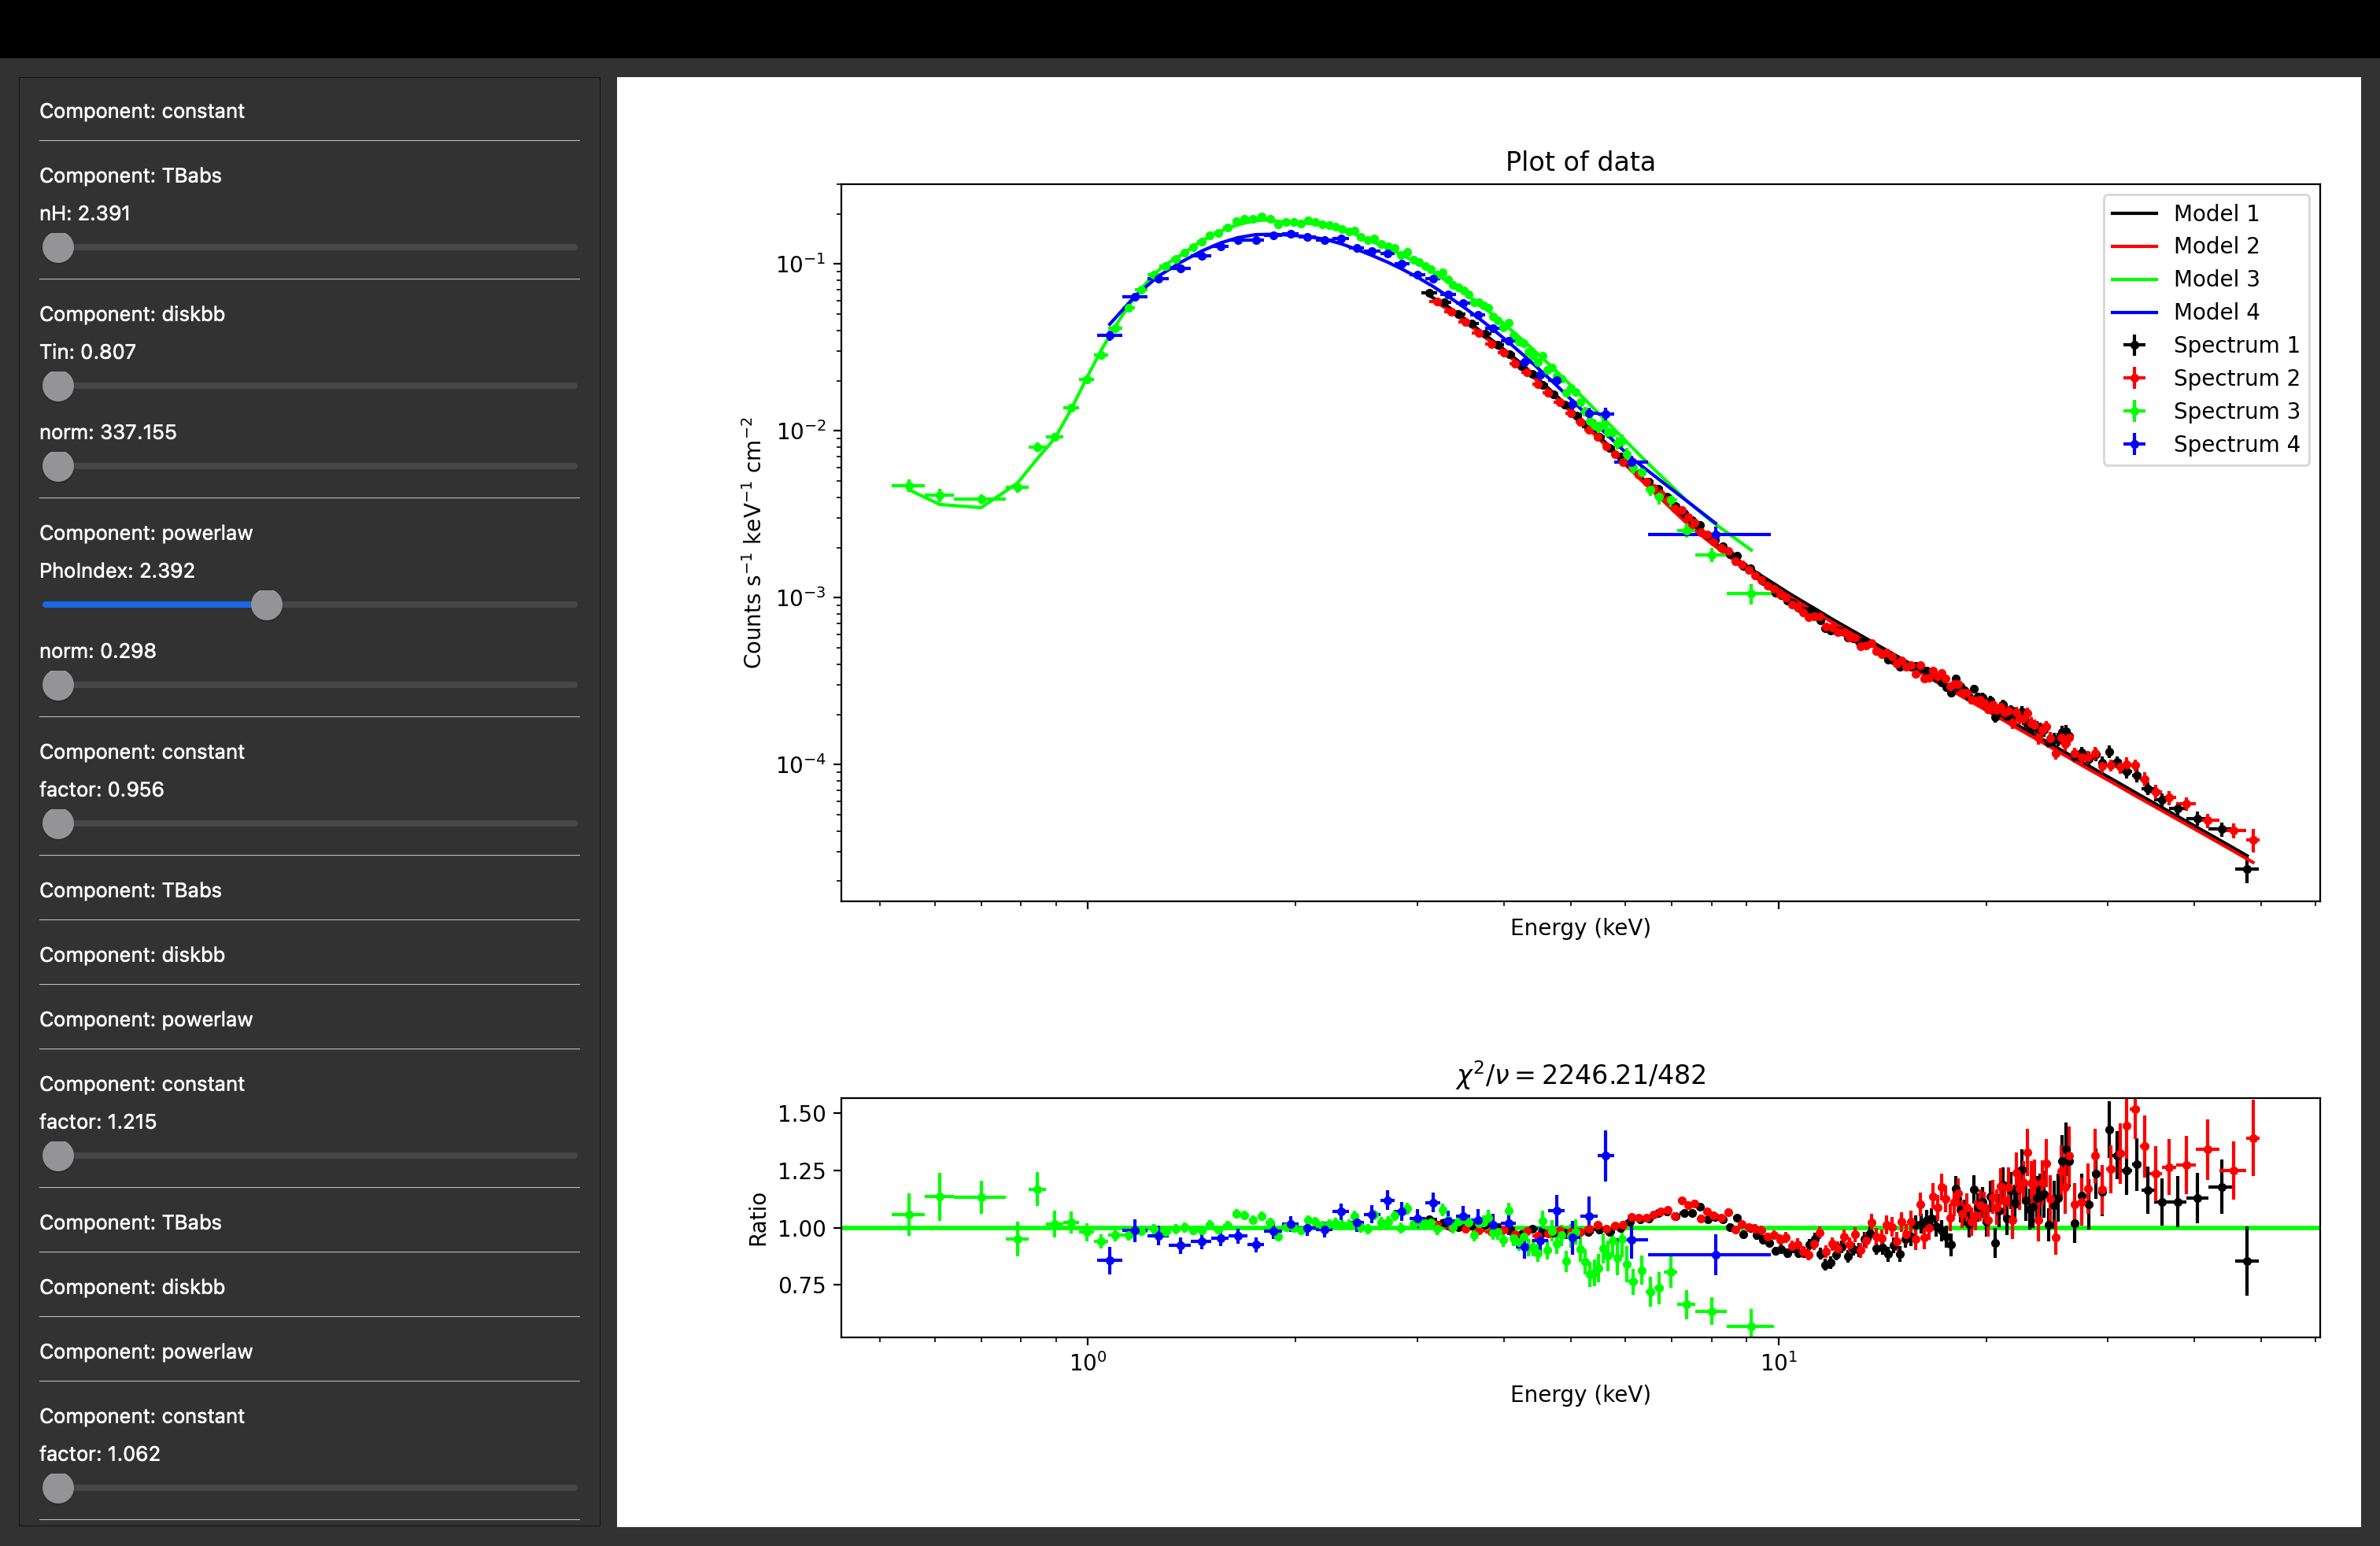
\includegraphics[width=0.7\linewidth]{documentation_images/plot_data_data+ratio.png}
    \caption{Data+ratio plot mode.}
\end{figure}

\begin{figure}[H]
    \centering
    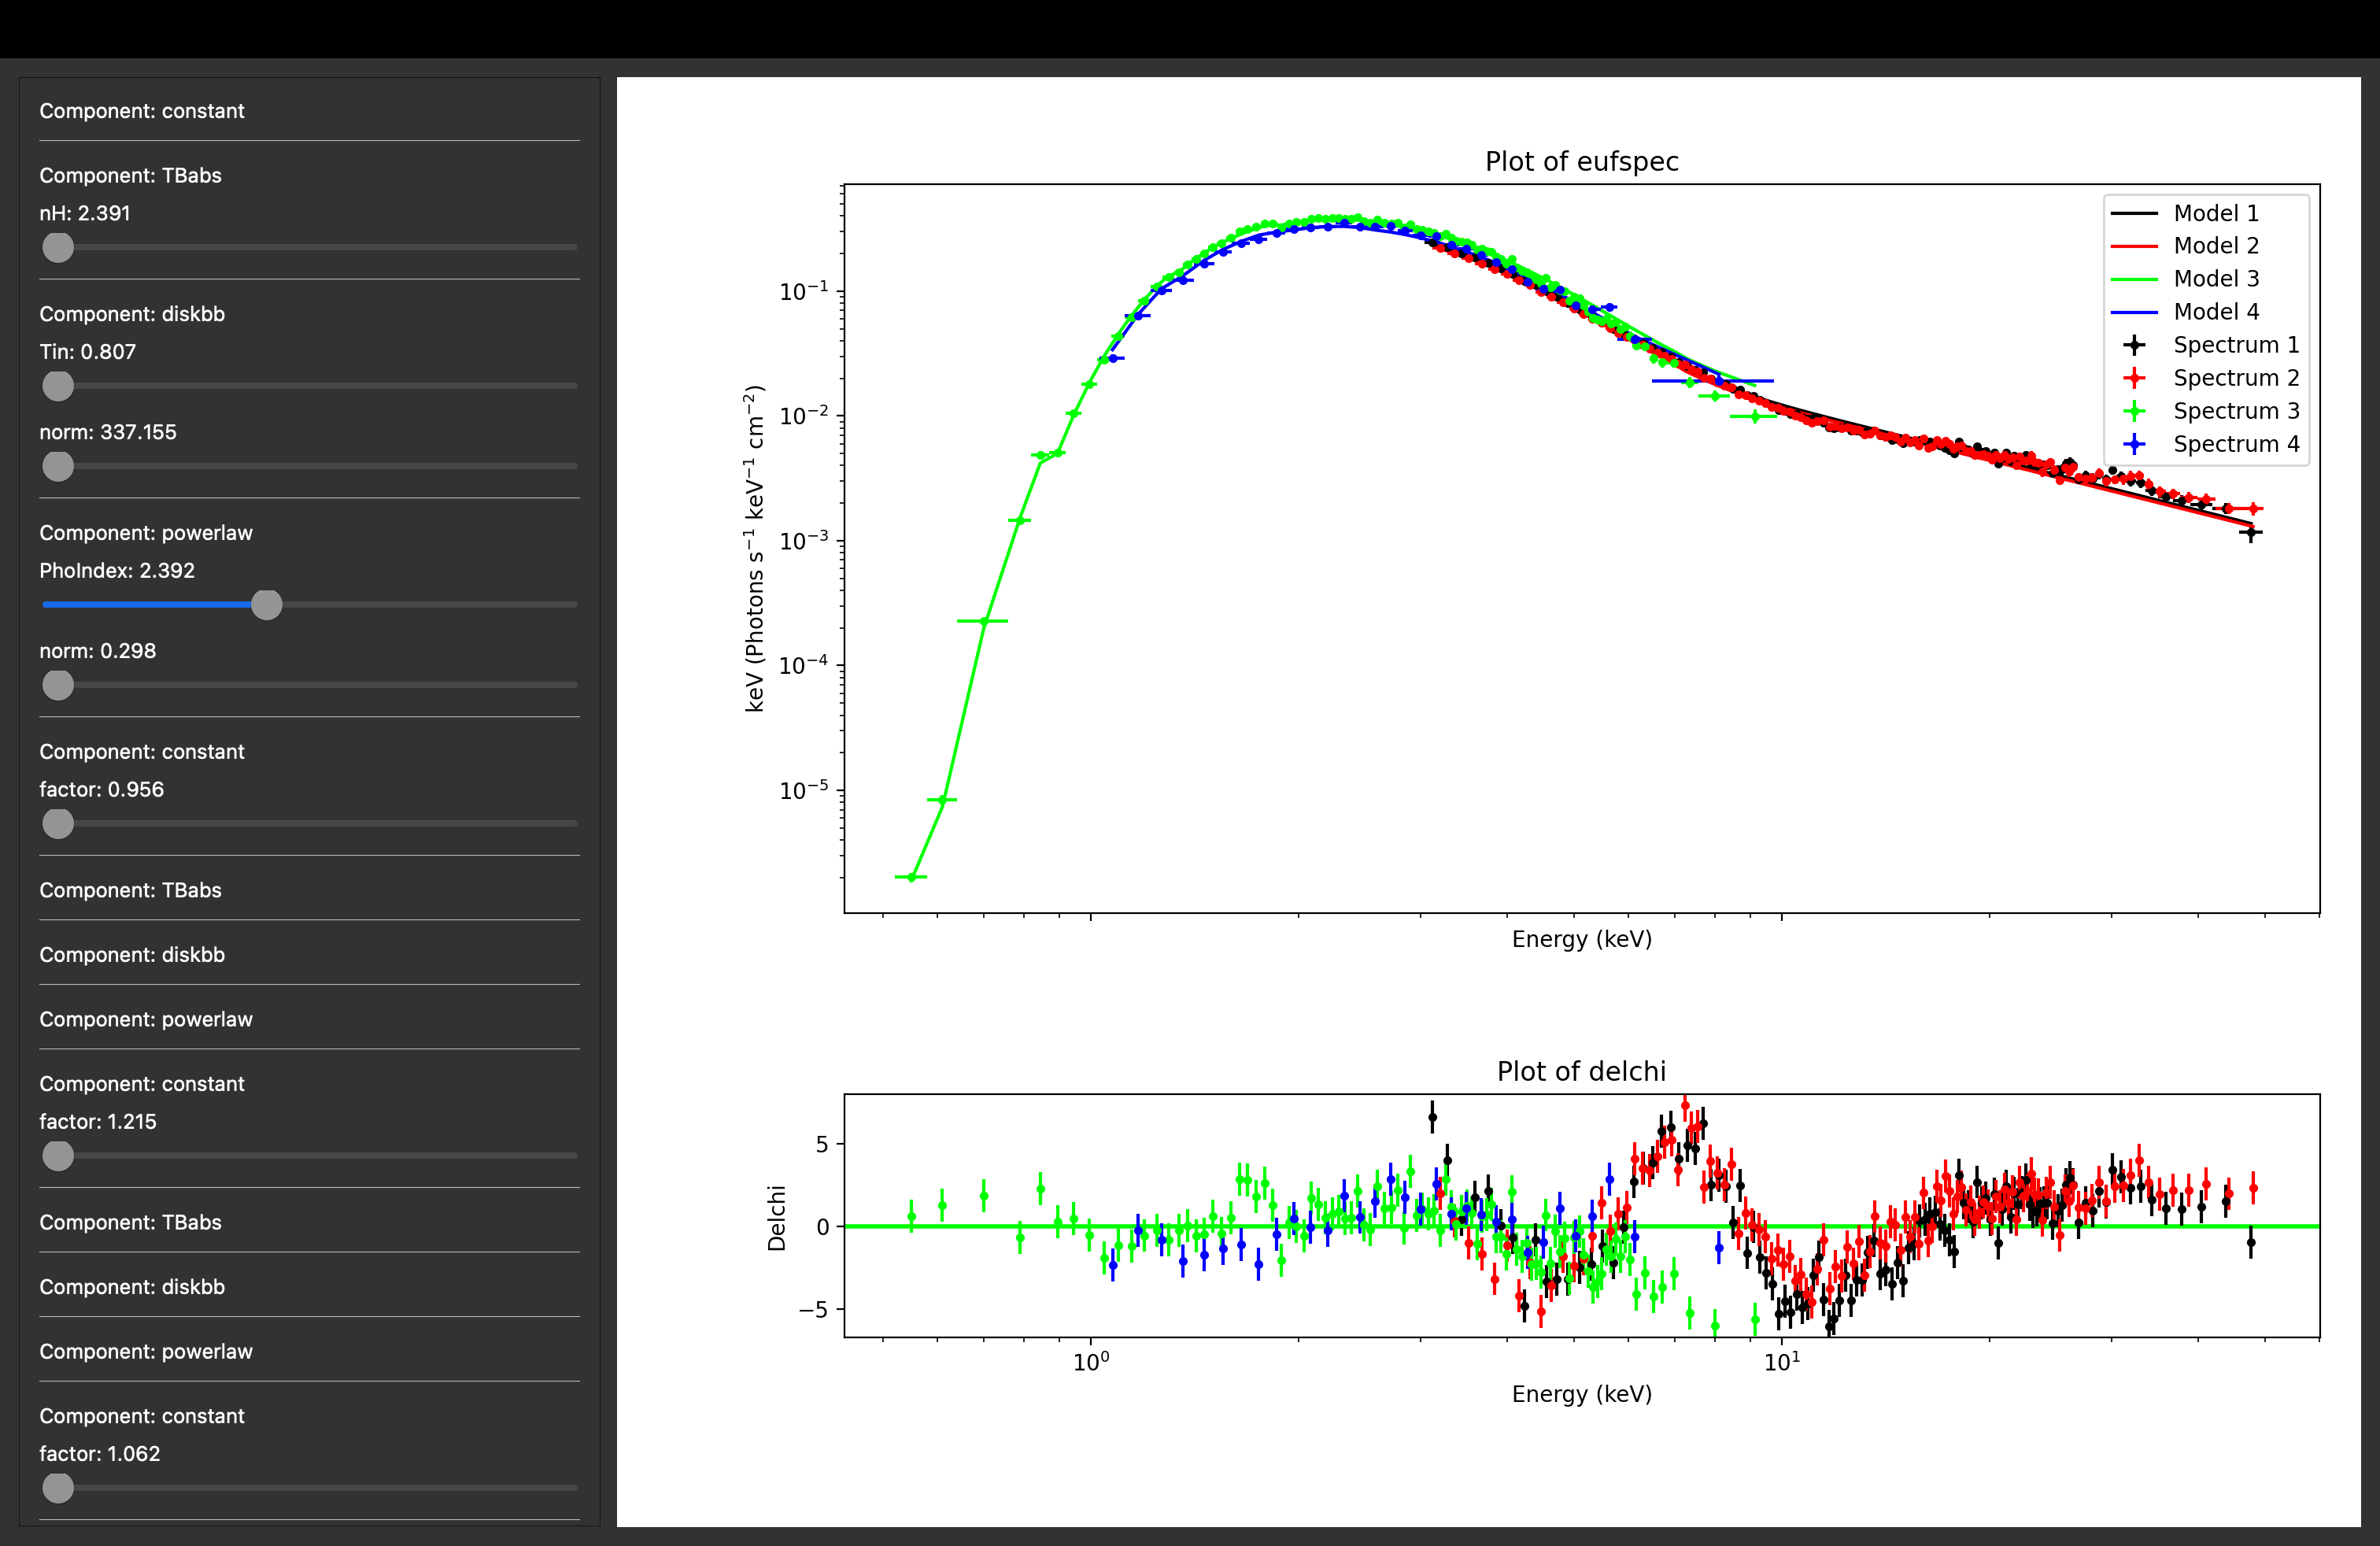
\includegraphics[width=0.7\linewidth]{documentation_images/plot_data_eufspec+delchi.png}
    \caption{Unfolded spectrum + delchi plot mode.}
\end{figure}

\begin{figure}[H]
    \centering
    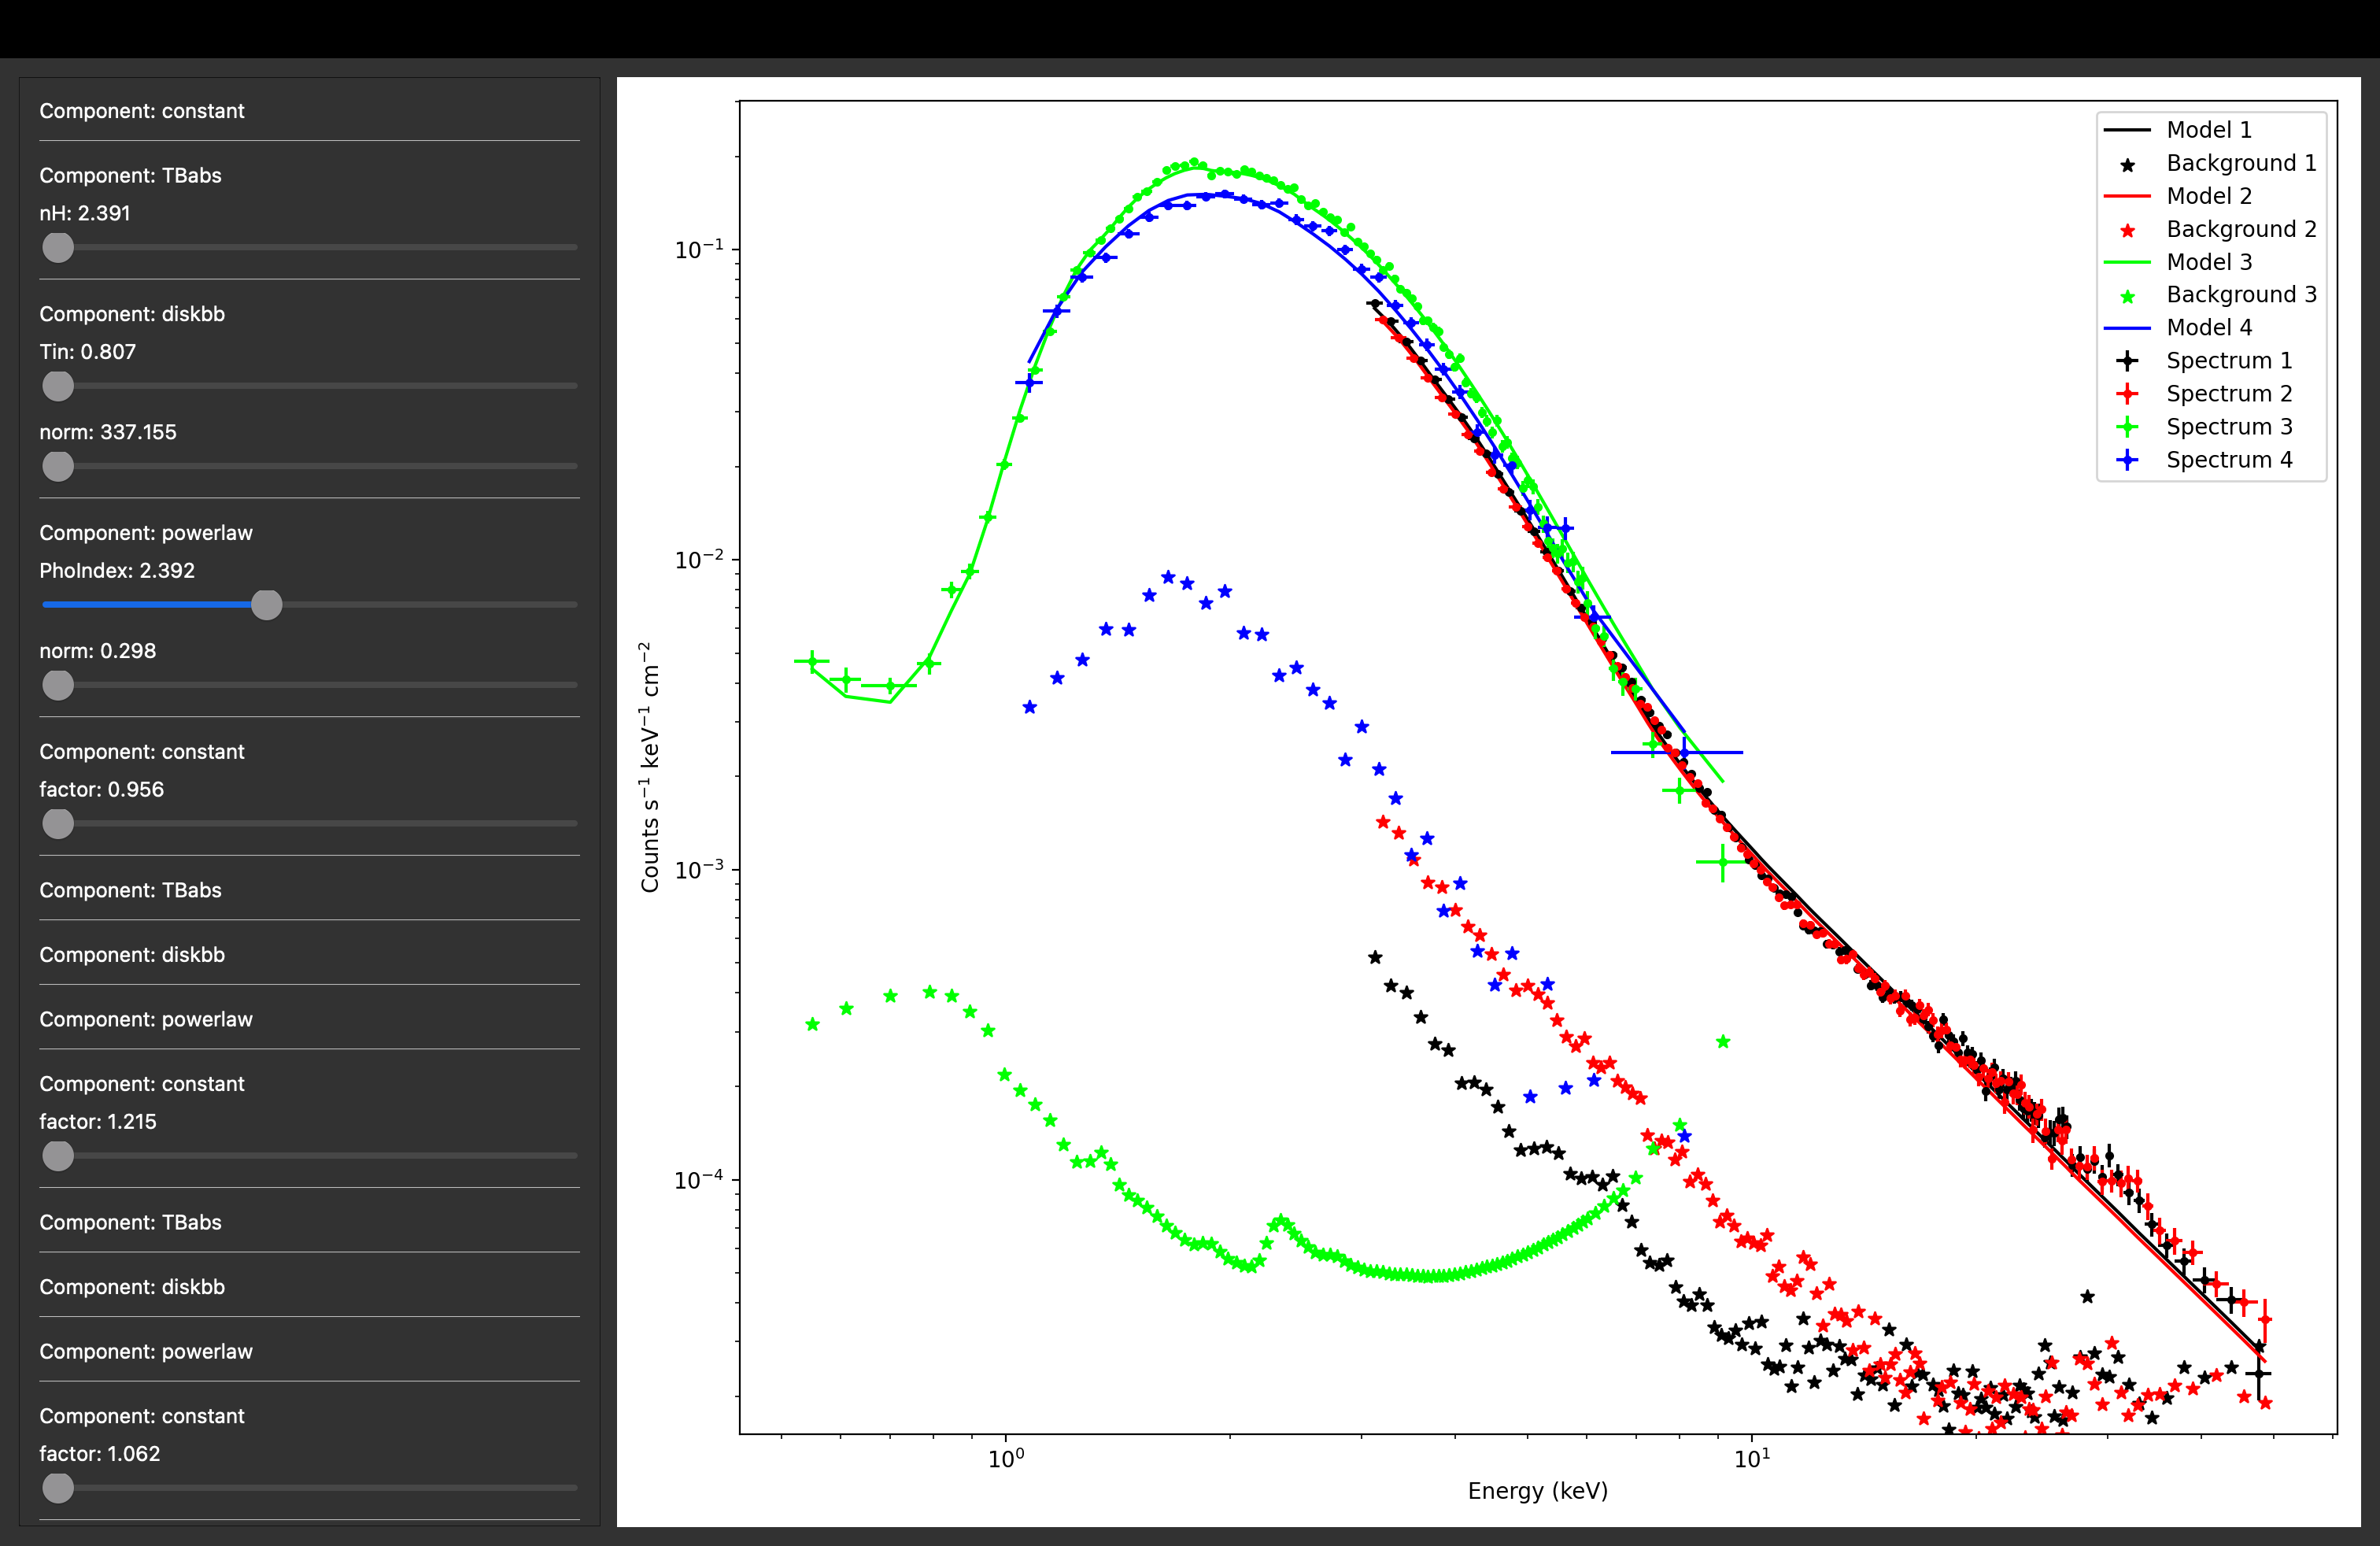
\includegraphics[width=0.7\linewidth]{documentation_images/include_background.png}
    \caption{Option to include or exclude background in the plot.}
\end{figure}

\section*{Saving and Exporting}

\begin{itemize}
    \item \textbf{File $\rightarrow$ Save Parameters as XCM:} Export the current model setup.
    \item \textbf{File $\rightarrow$ Save Plot:} Save the currently displayed plot to a PNG file.
    \item \textbf{File $\rightarrow$ Load Plot Style File:} Import a custom \texttt{.mplstyle} configuration for plot styling.
\end{itemize}

\section*{Additional Notes}

\begin{itemize}
    \item The software currently supports fitting loaded data via the \textbf{Perform Fit} option in the Plot menu.
    \item Default XSPEC fit settings are used unless otherwise modified.
    \item All parameter updates are immediately reflected in the XSPEC backend.
\end{itemize}

\begin{figure}[H]
    \centering
    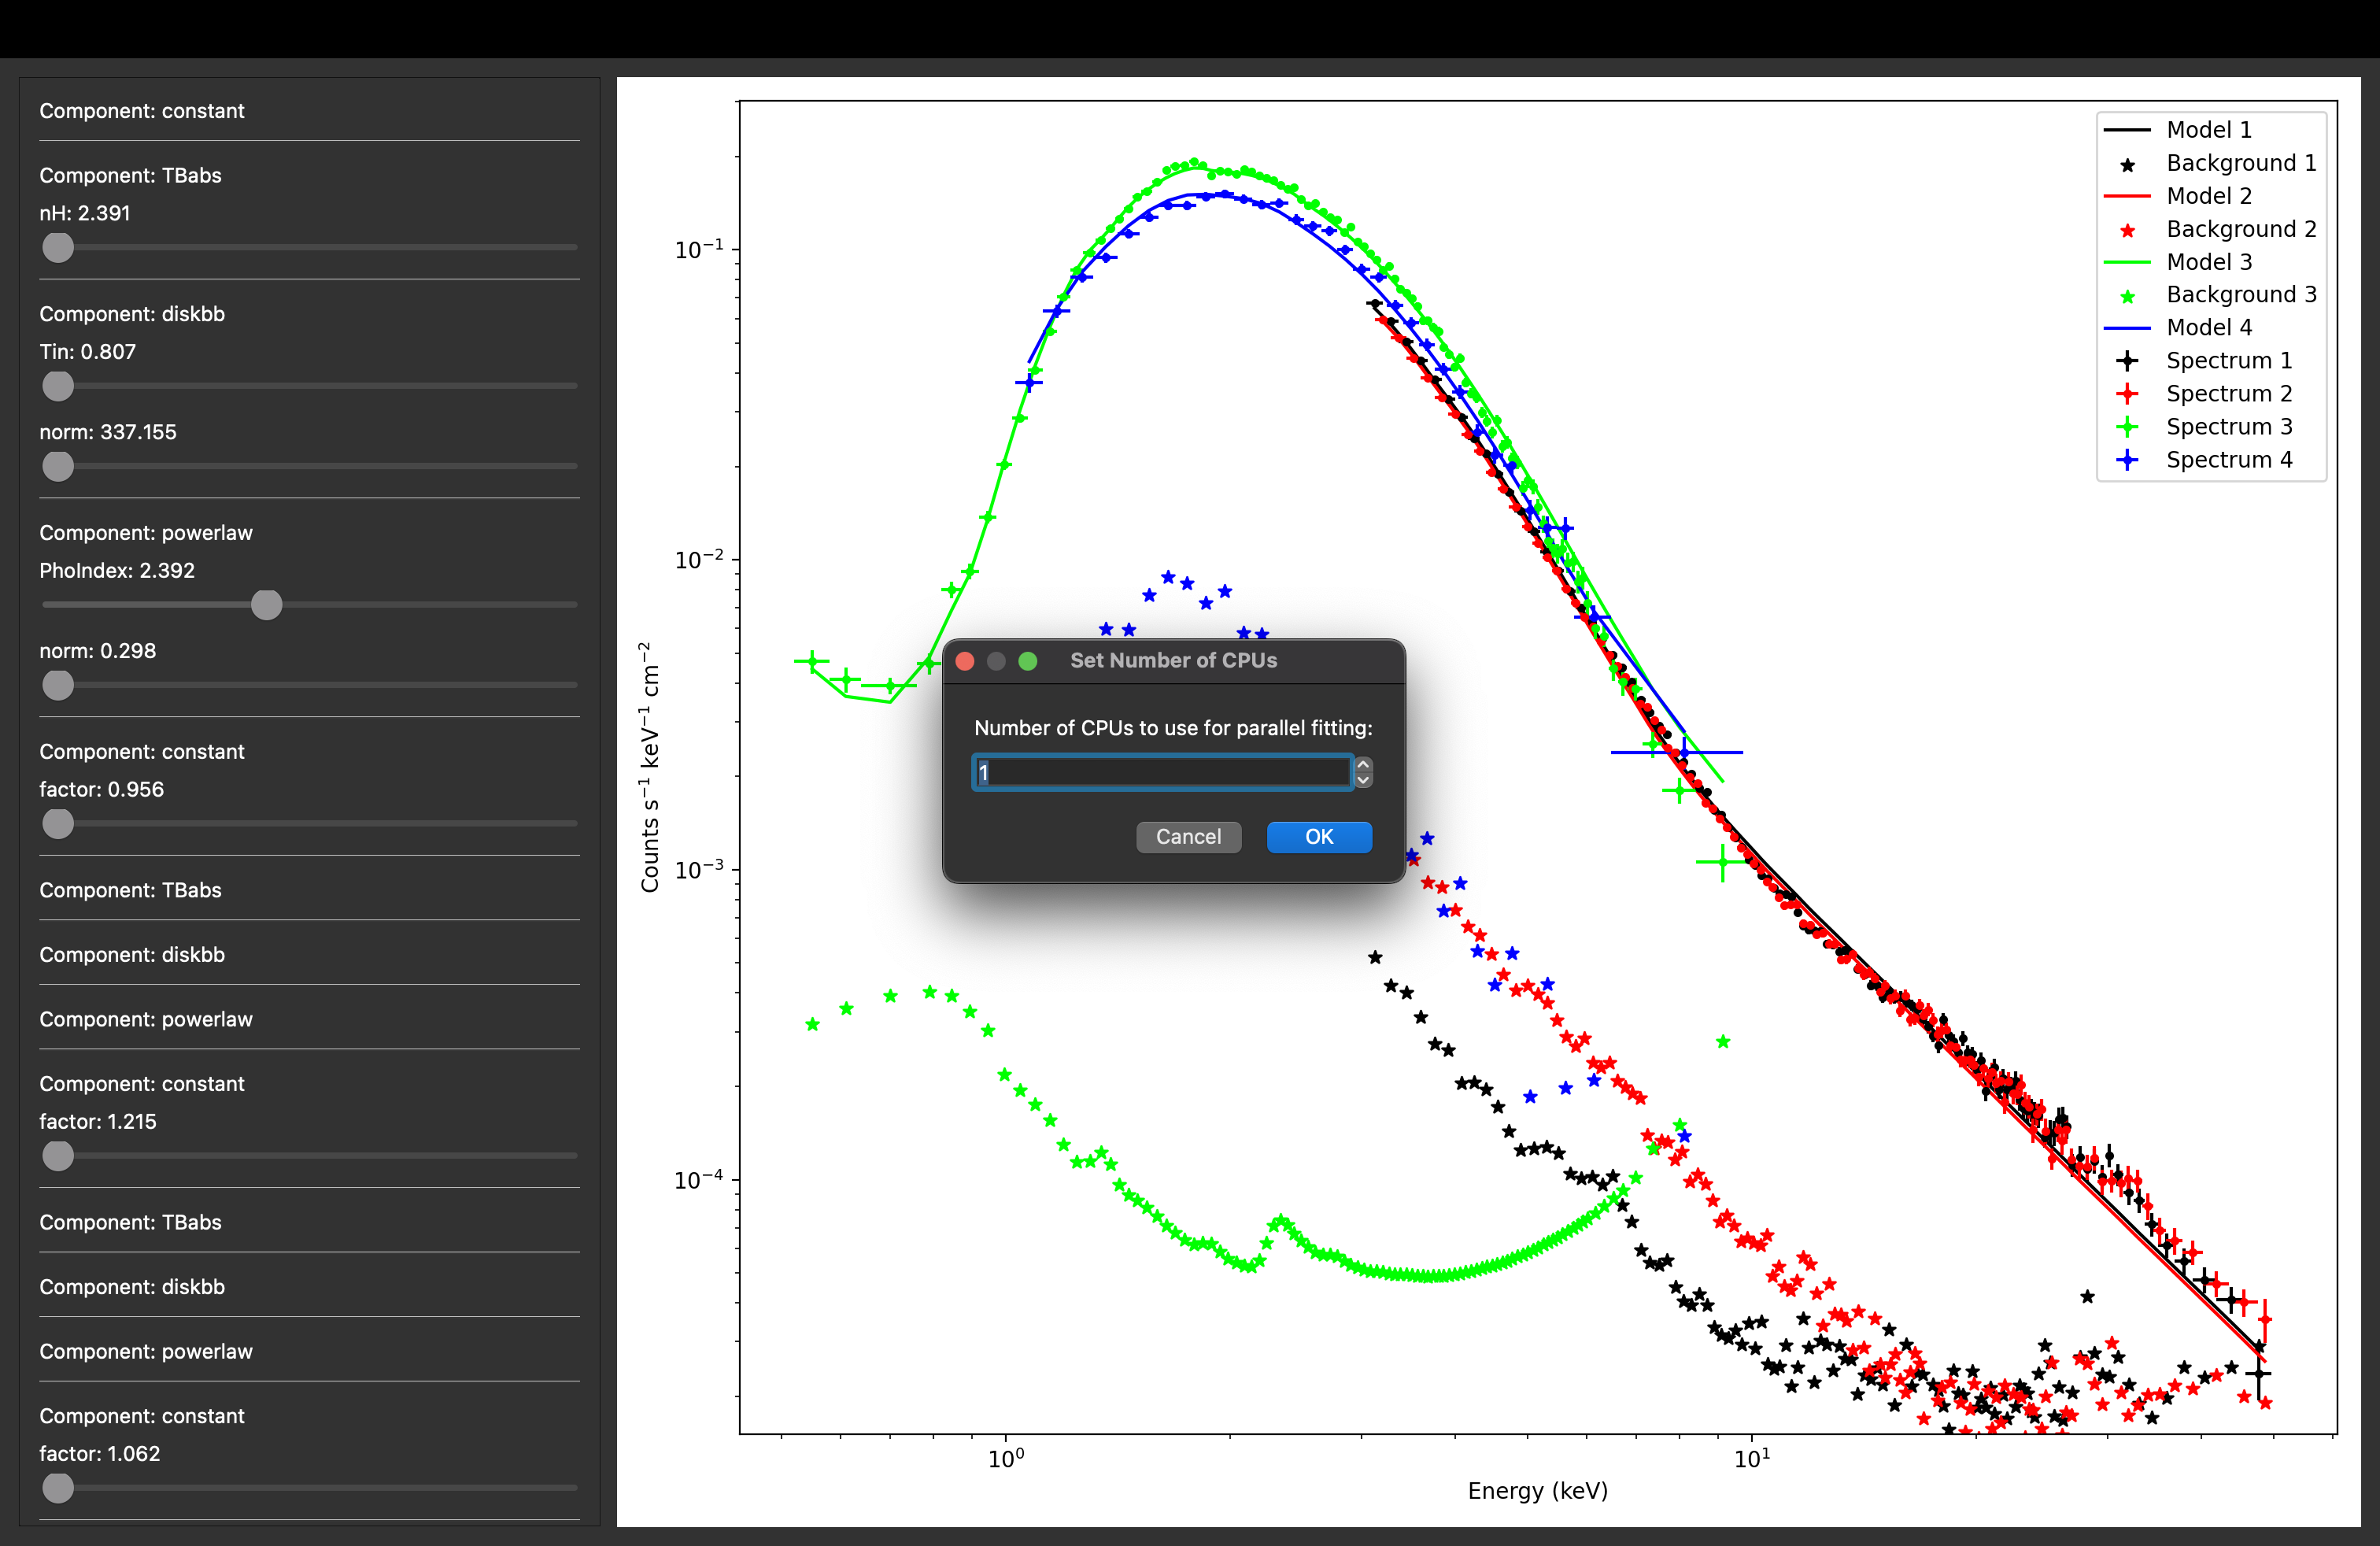
\includegraphics[width=0.7\linewidth]{documentation_images/set_number_of_cpus_for_parallel_fitting.png}
    \caption{Setting the number of CPUs for parallel fitting.}
\end{figure}

\section*{Future Work}

We are actively developing new features, including:
\begin{itemize}
    \item A fitting assistant for user-guided $\chi^2$ minimization (\textit{hence the name -- ChiByEye}).
    \item Advanced residual diagnostics.
    \item Support for time-resolved and multi-spectral fits.
\end{itemize}

\section*{Feedback and Contributions}

If you encounter bugs, want to suggest new features, or simply have feedback about usability, we would love to hear from you!  
This is an early-release version of \textbf{ChiByEye}, and we appreciate any help in improving it.

\section*{Acknowledgments}

This project was developed by:

\begin{itemize}
    \item \textbf{Paulo Silva} – Massachusetts Institute of Technology
    \item \textbf{Paul Draghis} – Massachusetts Institute of Technology
\end{itemize}

\bigskip

\noindent We acknowledge the developers of XSPEC and the creators of the relxill models for making this work possible.

\end{document}